%%% File encoding: UTF-8
%%% äöüÄÖÜß  <-- keine deutschen Umlaute hier? UTF-faehigen Editor verwenden!

%%% Magic Comments zum Setzen der korrekten Parameter in kompatiblen IDEs
% !TeX encoding = utf8
% !TeX program = pdflatex 
% !TeX spellcheck = de_DE
% !BIB program = biber

\documentclass[master,german]{hgbthesis}
% Zulässige Optionen in [..]: 
%   Typ der Arbeit: diploma, master (default), bachelor, internship 
%   Hauptsprache: german (default), english
%%%----------------------------------------------------------

\RequirePackage[utf8]{inputenc}		% bei der Verw. von lualatex oder xelatex entfernen!

\graphicspath{{images/}}    % Verzeichnis mit Bildern und Grafiken
\logofile{logo}				% Logo-Datei = images/logo.pdf (\logofile{}, wenn kein Logo gewünscht)
\bibliography{references}  	% Biblatex-Literaturdatei (references.bib)

%%%----------------------------------------------------------
% Angaben für die Titelei (Titelseite, Erklärung etc.)
%%%----------------------------------------------------------

%%% Einträge für ALLE Arbeiten: -----------------------------
\title{Partielle Lösungen zur allgemeinen Problematik}
\author{Peter A.\ Schlaumeier}
\programname{Universal Computing}
\placeofstudy{Hagenberg}
\dateofsubmission{2017}{02}{28}	% {YYYY}{MM}{DD}

%%% Zusätzlich für eine Bachelorarbeit: ---------------------
\thesisnumber{XXXXXXXXXX-A}   % Stud-ID, z.B. 1310238045-A  
% (A = 1. Bachelorarbeit)
\semester{Sommersemester 2016} 
\coursetitle{Einführung in die Tiefere Problematik 1} 
\advisor{Alois B.~Treuer, Päd.\ Phil.}

%%% Restriktive Lizenformel anstatt CC (nur für Typ master) -
%\strictlicense

%%%----------------------------------------------------------
\begin{document}
%%%----------------------------------------------------------

%%%----------------------------------------------------------
\frontmatter                    % Titelei (röm. Seitenzahlen)
%%%----------------------------------------------------------

\maketitle
\tableofcontents

\chapter{Vorwort}

 % Optional. Ggf. weglassen
\chapter{Kurzfassung}

\begin{german}
An dieser Stelle steht eine Zusammenfassung der Arbeit in Deutsch.
\end{german}		
\chapter{Abstract}


The proposed work describes a method for pose estimation of articulated objects without any prior knowledge of their body parts. Most existing pose estimation methods take advantage of trackers, and user inputs to estimate the joint positions. However, a completely unsupervised method constitutes an enormous potential but also a great challenge. A main solution to that is proposed by template matching associated with the non-rigid registration of meshes, which requires two poses of the same object and applies the Expectation-Maximization algorithm to segment the object into its rigid parts. This is done iteratively by assigning mesh points on body parts and finding transformations that perfectly match those body parts on both meshes. Based on this approach, a segmentation method is developed to obtain the rigid parts of an object and consequently estimate its joints.

			

%%%----------------------------------------------------------
\mainmatter          % Hauptteil (ab hier arab. Seitenzahlen)
%%%----------------------------------------------------------

\chapter{Einleitung}
\label{cha:Einleitung}


\chapter{Die Abschlussarbeit}
\label{cha:Abschlussarbeit}

Jede Abschlussarbeit%
\footnote{Die meisten der folgenden Bemerkungen gelten gleichsam für Bachelor-, Master- und Diplomarbeiten.} 
ist anders und dennoch sind sich gute
Arbeiten in ihrer Struktur meist sehr ähnlich, \va\ bei
technisch-natur\-wissen\-schaft\-lichen Themen. 

\section{Elemente der Abschlussarbeit}

Als Ausgangspunkt bewährt hat sich der folgende Grundaufbau, der natürlich 
vari\-iert und beliebig verfeinert werden kann:
%
\begin{enumerate}
\item \textbf{Einführung und Motivation}: Was ist die Problem- oder Aufgabenstellung und
warum sollte sich jemand dafür interessieren?
\item \textbf{Präzisierung des Themas}: Hier wird der aktuelle Stand der Technik
oder Wissenschaft ("`State-Of-The-Art"') beschrieben, es werden bestehende
Defizite oder offene Fragen aufgezeigt und daraus die
Stoßrichtung der eigenen Arbeit entwickelt.
\item \textbf{Eigener Ansatz}: Das ist natürlich der Kern der Arbeit. Hier
wird gezeigt, wie die vorher beschriebene Aufgabenstellung gelöst und --
häufig in Form eines Programms%
\footnote{\emph{Prototyp} ist in diesem Zusammenhang ein gerne benutzter Begriff, der im Deutschen
allerdings oft unrichtig dekliniert wird. Richtig ist: der \emph{Prototyp}, des \emph{Prototyps}, dem/den \emph{Protototyp} -- falsch hingegen \zB: des \emph{Prototyp\underline{en}}!
} --
realisiert wird, ergänzt durch illustrative Beispiele.
\item \textbf{Zusammenfassung}: Was wurde erreicht und welche Ziele sind
noch offen geblieben, wo könnte weiter gearbeitet werden?
\end{enumerate}
%
Natürlich ist auch ein gewisser dramaturgischer Aufbau der Arbeit
wichtig, wobei zu bedenken ist, dass der Leser in der Regel nur
wenig Zeit hat und -- anders als etwa bei einem Roman -- seine
Geduld nicht auf die lange Folter gespannt werden darf. Erklären
Sie bereits in der Einführung (und nicht erst im letzten Kapitel),
wie Sie an die Sache herangehen, welche Lösungen Sie vorschlagen
und wie erfolgreich Sie damit waren.

Übrigens, auch Fehler und Sackgassen dürfen (und sollten)
beschrieben werden; ihre Kenntnis hilft oft doppelte Experimente und
weitere Fehler zu vermeiden und ist damit sicher nützlicher als
jede Schönfärberei.
Und natürlich ist es auch nicht verboten, seine eigene Meinung 
in sachlicher Form zu äußern.


\section{Arbeiten in Englisch}
\label{sec:englisch}

Diese Vorlage ist zunächst darauf abgestellt, dass die
Abschlussarbeit in deutscher Sprache erstellt wird. Vor allem bei
Arbeiten, die in Zusammenarbeit mit größeren Firmen oder
internationalen Instituten entstehen, ist es häufig erwünscht,
dass die Abschlussarbeit zu besseren Nutzbarkeit in englischer
Sprache verfasst wird, und viele Hochschulen%
\footnote{Die FH Oberösterreich macht hier keine Ausnahme. 
Der Begriff "`Fachhochschule"' wird dabei entweder gar nicht
übersetzt oder -- wie im deutschsprachigen Raum mittlerweile üblich -- 
mit \emph{University of Applied Sciences}.
%Die offizielle englische Übersetzung von "`Medientechnik und -design"'
%ist übrigens \emph{Media Technology and Design}.
} 
lassen dies in
der Regel auch zu.

Beachtet sollte allerdings werden, dass das Schreiben dadurch nicht
einfacher wird, auch wenn einem Worte und Sätze im Englischen
scheinbar leichter "`aus der Feder"' fließen. Gerade im Bereich
der Informatik erscheint durch die Dominanz englischer
Fachausdrücke das Schreiben im Deutschen mühsam und das Ausweichen
ins Englische daher besonders attraktiv. Das ist jedoch
trügerisch, da die eigene Fertigkeit in der Fremdsprache
(trotz der meist langjährigen Schulbildung) häufig überschätzt wird.
Prägnanz und Klarheit gehen leicht verloren und bisweilen ist das
Resultat ein peinliches Gefasel ohne Zusammenhang und soliden
Inhalt. Sofern die eigenen Englischkenntnisse nicht wirklich gut sind, ist
es ratsam, zumindest die wichtigsten Teile der Arbeit zunächst in
Deutsch zu verfassen und erst nachträglich zu übersetzen. Besondere Vorsicht ist bei der Übersetzung von scheinbar
vertrauten Fachausdrücken angebracht. Zusätzlich ist es immer zu
empfehlen, die fertige Arbeit von einem "`native speaker"'
korrigieren zu lassen.



Technisch ist, außer der Spracheinstellung und den
unterschiedlichen Anführungszeichen (s.\
Abschn.~\ref{sec:anfuehrungszeichen}), für eine englische Arbeit
nicht viel zu ändern, allerdings sollte Folgendes beachtet werden:
%
\begin{itemize}
\item  Die Titelseite (mit der Bezeichnung "`Diplomarbeit"' oder "`Masterarbeit"') 
ist für die einzureichenden Exemplare jedenfalls in \emph{deutsch} zu halten,
auch wenn der Titel englisch ist. 
\item Ebenso muss neben dem
englischen \emph{Abstract} auch eine deutsche \emph{Kurzfassung}
enthalten sein. %
\item Akademische Titel von Personen haben im Englischen offenbar
weniger Bedeutung als im Deutschen und werden daher meist
weggelassen.
\end{itemize}

\chapter{Zum Arbeiten mit \latex}
\label{cha:ArbeitenMitLatex}


\chapter{Abbildungen, Tabellen, Quellcode}
\label{cha:Abbildungen}



\chapter[Mathem.\ Formeln etc.]{Mathematische Formeln, Gleichungen und Algorithmen}
\label{cha:Mathematik}



Das Formatieren von mathematischen Elementen gehört sicher zu den
Stär\-ken von \latex. Man unterscheidet zwischen mathematischen Elementen
im Fließtext und freistehenden Gleichungen, die in der Regel
fortlaufend nummeriert werden. Analog zu Abbildungen und Tabellen sind dadurch
Querverweise zu Gleichungen leicht zu realisieren.
Hier nur einige Beispiele und spezielle Themen, vieles weitere dazu findet sich \zB in
\cite[Kap.\ 7]{Kopka2003} und~\cite{Voss2014}.


\section{Mathematische Elemente im Fließtext}

Mathematische Symbole, Ausdrücke, Gleichungen etc.\ werden im Fließtext durch paarweise 
\verb!$! \ldots \verb!$! markiert. Hier ein simples Beispiel:
%
\begin{itemize}
\item[]
Der Nah-Unendlichkeitspunkt liegt bei
$\bar{a} = f' \cdot (f' / (K \cdot u_{\max}) + 1)$,
sodass bei einem auf $\infty$ eingestellten Objektiv von der Entfernung
$\bar{a}$ an alles scharf ist. Fokussiert man das
Objektiv auf die Entfernung $\bar{a}$ (\dah, $a_0 = \bar{a}$), dann wird
im Bereich $[\frac{\bar{a}}{2}, \infty]$ alles scharf.
\end{itemize}
%
Dabei sollte unbedingt darauf geachtet werden, dass die Höhe der einzelnen Elemente im Text nicht zu groß wird. 

\paragraph{Häufiger Fehler:} 
Im Fließtext wird bei einfachen Variablen oft auf die Verwendung der richtigen, mathematischen
Zeichen vergessen, wie etwa in "`X-Achse"' anstelle von "`$X$-Achse"' (\verb!$X$-Achse!).

\paragraph{Zeilenumbrüche:}
Bei längeren mathematischen Elementen im Fließtext sind Probleme mit Zeilenumbrüchen
vorprogrammiert. In der Regel ermöglicht \latex nur am "`="' einen Zeilenumbruch,
an anderer Stelle kann man Umbrüche mit \texttt{{\bs}allowbreak} ermöglichen. 
Hier ein kleines Beispiel:
%
\begin{itemize}
\item[a)] Einen einfachen Zeilenvektor definiert man beispielsweise in der Form 
		$\boldsymbol{x} = (x_0, x_1, \ldots, x_{n-1})$.
\item[b)] Einen einfachen Zeilenvektor definiert man beispielsweise in der Form 
	$\boldsymbol{x} = (x_0,\allowbreak x_1,\allowbreak\ldots,\allowbreak x_{n-1})$.
\end{itemize}
Die Zeile in a) sollte über den Seitenrand hinauslaufen, b) hingegen enthält
\texttt{{\bs}allowbreak} an mehreren Stellen und sollte daher sauber umbrechen.


\section{Freigestellte Ausdrücke}

Freigestellte mathematische Ausdrücke können in \latex\ im einfachsten Fall durch paarweise 
\verb!$$! \ldots \verb!$$! erzeugt werden. Das Ergebnis wird zentriert, erhält jedoch keine 
Nummerierung. So ist \zB\ $$y = 4 x^2$$ das Ergebnis von \verb!$$y = 4 x^2$$!.


\subsection{Einfache Gleichungen} 

Meistens wird in solchen Fällen jedoch die \texttt{equation}-Umgebung zur Herstellung nummerierter 
Gleichungen verwendet, auf die im Text jederzeit verwiesen werden kann. Zum Beispiel erzeugt
%
\begin{LaTeXCode}[numbers=none]
\begin{equation}
  f(k) = \frac{1}{N} \sum_{i=0}^{k-1} i^2 . 
  \label{eq:MyFirstEquation}
\end{equation}
\end{LaTeXCode}
%
die Gleichung
%
\begin{equation}
  f(k) = \frac{1}{N} \sum_{i=0}^{k-1} i^2 . 
\label{eq:MyFirstEquation}
\end{equation}
%
Mit \verb!\ref{eq:MyFirstEquation}! erhält man wie üblich die Nummer (\ref{eq:MyFirstEquation}) dieser Gleichung (siehe dazu auch Abschn.\ \ref{sec:VerweiseAufGleichungen}). 
Dieselbe Gleichung \emph{ohne} Nummerierung kann übrigens mit der \texttt{equation*}-Umgebung erzeugt werden.



\begin{center}
\setlength{\fboxrule}{0.2mm}
\setlength{\fboxsep}{2mm}
\fbox{%
\begin{minipage}{0.9\textwidth}
Man beachte, dass \textbf{Gleichungen} inhaltlich ein \textbf{Teil des Texts} sind und daher neben der sprachlichen
\textbf{Überleitung} auch die \textbf{Interpunktion} (wie in Gl.\ \ref{eq:MyFirstEquation} gezeigt) beachtet werden muss. 
Bei Unsicherheiten sollte man sich passende Beispiele in einem guten Mathematik\-buch ansehen.
\end{minipage}}
\end{center}
%
Für Interessierte findet sich mehr zum Thema Mathematik und Prosa in \cite{Mermin1989} und \cite{Higham1998}.

\subsection{Mehrzeilige Gleichungen}

Für mehrzeilige Gleichungen bietet \latex\ die 
\verb!eqnarray!-Umgebung, die allerdings etwas eigenwillige Zwischenräume erzeugt.
Es empfiehlt sich, dafür gleich auf die erweiterten Möglichkeiten des \texttt{amsmath}-Pakets%
\footnote{American Mathematical Society (AMS). \texttt{amsmath} ist Teil der \latex\ Standardinstallation und wird von \texttt{hgb.sty} bereits importiert.}
\cite{Mittelbach2016} zurückzugreifen.
Hier ein Beispiel mit zwei am $=$ Zeichen ausgerichteten Gleichungen,
%
\begin{align}
f_1 (x,y) &= \frac{1}{1-x} + y , \label{eq:f1} \\
f_2 (x,y) &= \frac{1}{1+y} - x , \label{eq:f2}
\end{align}
%
erzeugt mit der \texttt{align}-Umgebung aus dem \texttt{amsmath}-Paket:
%
\begin{LaTeXCode}[numbers=none]
\begin{align}
  f_1 (x,y) &= \frac{1}{1-x} + y , \label{eq:f1} \\
  f_2 (x,y) &= \frac{1}{1+y} - x , \label{eq:f2}
\end{align}
\end{LaTeXCode}


\subsection{Fallunterscheidungen}

Mit der \texttt{cases}-Umgebung aus \texttt{amsmath} sind Fallunterscheidungen, \ua\ innerhalb von Funktionsdefinitionen, sehr einfach zu bewerkstelligen. Beispielsweise wurde die rekursive Definition
%
\begin{equation}
	f(i) =
	\begin{cases}
	  0             & \text{für $i = 0$,}\\
	  f(i-1) + f(i) & \text{für $i > 0$.}
	\end{cases}
\end{equation}
mit folgenden Anweisungen erzeugt:
%
\begin{LaTeXCode}[numbers=none]
\begin{equation}
	f(i) =
	\begin{cases}
	  0             & \text{für $i = 0$,}\\
	  f(i-1) + f(i) & \text{für $i > 0$.}
	\end{cases}
\end{equation}
\end{LaTeXCode}
%
Man beachte dabei die Verwendung des sehr praktischen \verb!\text{..}!-Makros, mit dem im Mathematik-Modus gewöhnlicher Text eingefügt werden kann, sowie wiederum die Interpunktion innerhalb der Gleichung.


\subsection{Gleichungen mit Matrizen}

Auch hier bietet \texttt{amsmath} einige Vorteile gegenüber der Verwendung der \latex\ Standardkonstrukte. Dazu ein einfaches Beispiel für die Verwendung der \texttt{pmatrix}-Umgebung für Vektoren und Matrizen,
%
\begin{equation}
	\begin{pmatrix} x' \\ y' \end{pmatrix}
	= 
	\begin{pmatrix}
	  \cos \phi & -\sin \phi \\
	  \sin \phi & \phantom{-}\cos \phi
	\end{pmatrix} 
	\cdot
	\begin{pmatrix}	x \\ y \end{pmatrix} ,
\end{equation}
%
das mit den folgenden Anweisungen erzeugt wurde:
%
\begin{LaTeXCode}
\begin{equation}
	\begin{pmatrix} 
			x' \\ 
			y' 
	\end{pmatrix}
	= 
	\begin{pmatrix}
		  \cos \phi &           -\sin \phi \\
		  \sin \phi & \phantom{-}\cos \phi /+ \label{lin:phantom} +/
	\end{pmatrix} 
	\cdot
	\begin{pmatrix} 
			x \\ 
			y 
	\end{pmatrix} ,
\end{equation}
\end{LaTeXCode}
%
Ein nützliches Detail darin ist das \tex-Makro \verb!\phantom{..}! (in Zeile \ref{lin:phantom}), das sein Argument unsichtbar einfügt und hier als Platzhalter für das darüberliegende Minuszeichen verwendet wird. Alternativ zu \texttt{pmatrix} kann mit der \texttt{bmatrix}-Umgebung Matrizen
und Vektoren mit eckigen Klammern erzeugt werden.
Zahlreiche weitere mathematische Konstrukte des \texttt{amsmath}-Pakets sind in \cite{Mittelbach2016} beschrieben.

\begin{comment}
% Umsetzung ohne amsmath:
\begin{equation}
\left[ \begin{array}{c}
  x' \\ y'
\end{array} \right] 
= 
\left[ \begin{array}{rr}
	 \cos \phi & \sin \phi \\
	-\sin \phi & \cos \phi
\end{array} \right] 
\cdot
\left[ \begin{array}{c}
	x \\ y
\end{array}
\right] 
.
\end{equation}
\end{comment}



\subsection{Verweise auf Gleichungen}
\label{sec:VerweiseAufGleichungen}

Beim Verweis auf nummerierte Formeln und Gleichungen genügt grundsätzlich die Angabe 
der entsprechenden Nummer in runden Klammern,
\zB\
\begin{center}
%"`\ldots\ wie aus (\ref{eq:f1}) abgeleitet werden kann \ldots"'
"`\ldots\ wie aus (\ref{eq:f1}) abgeleitet werden kann \ldots"'
\end{center}
Um Missverständnisse zu vermeiden, sollte aber -- \va\ in Texten mit
nur wenigen mathematischen Elementen -- "`Gleichung \ref{eq:f1}"', "`Gl.~\ref{eq:f1}"' 
oder "`Gl.~(\ref{eq:f1})"' geschrieben werden (natürlich konsistent). 
%\emph{Falsch} wäre hingegen "`Gleichung (\ref{eqn:zerstreuungskreis})"'.

\begin{center}
\setlength{\fboxrule}{0.2mm}
\setlength{\fboxsep}{2mm}
\fbox{%
\begin{minipage}{0.9\textwidth}
\textbf{Achtung:} Vorwärtsverweise auf (im Text weiter hinten liegende) Gleichungen sind \textbf{äußerst ungewöhnlich} 
und sollten vermieden werden! Glaubt man dennoch so etwas zu benötigen, dann wurde
meistens ein Fehler in der Anordnung gemacht.
\end{minipage}}
\end{center}


\section{Spezielle Symbole}

Für einen Großteil der mathematischen Symbole werden spezielle Makros benötigt. Im Folgenden werden einige der gebräuchlichsten aufgelistet.

\subsection{Zahlenmengen}
Einige häufig verwendete Symbole sind leider im ursprünglichen
mathematischen Zeichensatz von \latex nicht enthalten, \zB die
Symbole für die reellen und natürlichen Zahlen. Im \texttt{hagenberg}-Paket sind diese Symbole als Makros 
%\verb!\R! ($\R$), \verb!\Z! ($\Z$), \verb!\N! ($\N$), \verb!\C! ($\C$) und \verb!\Q! ($\Q$)
\verb!\R!, \verb!\Z!, \verb!\N!, \verb!\Cpx!, \verb!\Q!
($\R, \Z, \N, \Cpx, \Q$)
mithilfe der \emph{AMS Blackboard Fonts} definiert, \zB:
\begin{center}
$x \in \R$ , $k \in \N_0$, $z = (a + \mathrm{i} \cdot b) \in \Cpx$.
\end{center}


\subsection{Operatoren}

In \latex\ sind Dutzende von mathematischen Operatoren für spezielle Anwendungen definiert. Am häufigsten werden natürlich die arithmetischen Operatoren $+$, $-$, $\cdot$ und $/$ benötigt. Ein dabei oft beobachteter Fehler (der wohl aus der Programmierpraxis resultiert) ist die Verwendung von $*$ für die einfache Multiplikation -- richtig ist $\cdot$ (\verb!\cdot!).%
\footnote{Das Zeichen $*$ ist üblicherweise für den \emph{Faltungsoperator} vorgesehen.}
%
Für Angaben wie \zB\ "`ein Feld mit $25 \times 70$ Metern"' (aber auch fast \emph{nur} dafür) wird sinnvollerweise der $\times$ (\verb!\times!) Operator und \emph{nicht} einfach das Textzeichen~"`x"' verwendet!


\subsection{Variable (Symbole) mit mehreren Zeichen}
Vor allem bei der mathematischen Spezifikation von Algorithmen und Programmen
ist es häufig notwendig, Symbole (Variablennamen) mit mehr als einem Zeichen
zu verwenden, \zB
%
$$Scalefactor\leftarrow Scalefactor^2 \cdot 1.5 \; ,$$
%
\textbf{fälschlicherweise} erzeugt durch 
\begin{quote}
	\verb!$Scalefactor \leftarrow Scalefactor^2! \verb!\cdot 1.5$!.
\end{quote}
Dabei interpretiert \latex allerdings die Zeichenkette "`Scalefactor"' als 11 einzelne,
aufeinanderfolgende Symbole $S$, $c$, $a$, $l$, $e$, \ldots und setzt dazwischen
entsprechende Abstände.
\textbf{Richtig} ist, diese Buchstaben mit
\verb!\mathit{..}! zu \emph{einem} Symbol zusammenzufassen.
Der Unterschied ist in diesem Fall deutlich sichtbar:
%
\begin{center}
\setlength{\tabcolsep}{4pt}
\begin{tabular}{llll}
\text{Falsch:}   & $Scalefactor^2$ & $\leftarrow$ & \verb!$Scalefactor^2$! \\
\text{Richtig:}  & $\mathit{Scalefactor}^2$ & $\leftarrow$ & \verb!$\mathit{Scalefactor}^2$!
\end{tabular}
\end{center}
%
Grundsätzlich sollten derart lange Symbolnamen aber ohnehin vermieden und stattdessen 
möglichst kurze (gängige) Symbole verwendet werden
(\zB\ Brennweite $f = 50 \, \mathrm{mm}$ statt $\mathit{Brennweite} = 50 \, \mathrm{mm}$).

\subsection{Funktionen}

Während Symbole für Variablen traditionell (und in \latex\ automatisch) \emph{italic} gesetzt werden, wird für die Namen von Funktionen und Operatoren üblicherweise
\emph{roman} als Schrifttyp verwendet, wie \zB in
\begin{center}
\begin{tabular}{lcl}
	$\sin \theta = \sin(\theta + 2 \pi)$ & 
	$\leftarrow$ & \verb!$\sin \theta = \sin(\theta + 2 \pi)$! \\
	\end{tabular}
\end{center}
Das ist bei den bereits vordefinierten Standardfunktionen (wie
\verb!\sin!,
\verb!\cos!,
\verb!\tan!,
\verb!\log!,
\verb!\max!
\uva) automatisch der Fall.
Diese Konvention sollte auch bei selbstdefinierten Funktionen befolgt werden,
wie etwa in
\begin{center}
	\begin{tabular}{lcl}
	$\mathrm{dist}(A,B) := |A-B|$ & $\leftarrow$ & 
	\verb!$\mathrm{dist}(A,B) := |A-B|$! \\
	\end{tabular}
\end{center}


\subsection{Maßeinheiten und Währungen}

Bei der Angabe von Maßeinheiten wird üblicherweise Normalschrift
(keine Italics) verwendet, \zB:
\begin{quote}
Die Höchstgeschwindigkeit der \textit{Bell XS-1} beträgt 345~m/s
bei einem Startgewicht von 15~t. 
Der Prototyp kostete über 25.000.000 US\$, also ca.\ 19.200.000 \euro\ nach heutiger Umrechnung.
\end{quote}
Der Abstand zwischen der Zahl und der Maßeinheit ist dabei
gewollt.
Das \$-Zeichen erzeugt wird mit \verb!\$! und
das Euro-Symbol (\euro) mit dem Makro \verb!\euro! erzeugt.%
\footnote{Das \euro\ Zeichen ist nicht im ursprünglichen \latex-Zeichensatz enthalten
sondern wird mit dem \texttt{eurosym}-Paket erzeugt.}


\subsection{Kommas in Dezimalzahlen (Mathematik-Modus)}

\latex\ setzt im Mathematik-Modus (also innerhalb von \verb!$$! oder in Gleichungen) nach dem angloamerikanischen Stil in Dezimalzahlen grundsätzlich den \emph{Punkt} (\verb!.!) als Trennsymbol voraus. So wird etwa mit \verb!$3.141$! normalerweise die Ausgabe "`3.141"' erzeugt. Um das in Europa übliche Komma in Dezimalzahlen zu verwenden, genügt es \emph{nicht}, einfach \verb!.! durch \verb!,! zu ersetzen. Das Komma wird in diesem Fall
als \textbf{Satzzeichen} interpretiert und sieht dann so aus:
\begin{quote}
\verb!$3,141$!	$\quad \rightarrow \quad 3,141$ 
\end{quote}
(man beachte den Leerraum nach dem Komma). Dieses Verhalten lässt sich in \latex\ zwar global umdefinieren, was aber wiederum zu einer Reihe unangenehmer Nebeneffekte führt. Eine einfache (wenn auch nicht sehr elegante) Lösung ist, Kommazahlen im Mathematik-Modus so zu schreiben:
\begin{quote}
\verb!$3{,}141$!	$\quad \rightarrow \quad 3{,}141$
\end{quote}



\subsection{Mathematische Werkzeuge}

Für die Erstellung komplizierter Gleichungen ist es mitunter
hilfreich, auf spezielle Software zurückzugreifen. Unter anderem können
aus dem Microsoft \emph{Equation Editor} und aus {\em
Mathematica} auf relativ einfache Weise \latex-An\-wei\-sun\-gen
für mathematische Gleichungen exportiert und direkt (mit etwas
manueller Nacharbeit) in das eigene \latex-Dokument übernommen werden.


\section{Algorithmen}

Für die Beschreibung von Algorithmen in mathematischer Form oder auch für
Pseudo\-code ist in \latex selbst keine spezielle Unterstützung vorgesehen.
Dazu gibt es jedoch eine Reihe von \latex-Paketen (\zB\ \texttt{algorithms}, 
\texttt{algorithmicx}, \texttt{algorithm2e}).
Das Beispiel in Alg.~\ref{alg:Example} wurde mit der Float-Umgebung \texttt{algorithm} 
und dem \texttt{algorithmicx}-Paket ausgeführt
(Quellcode in Prog.~\ref{prog:AlgExample}).


%%--------------------------------------------------------------------

\begin{algorithm}[tbp]
\caption{Bikubische Interpolation in 2D.
	$w_{\mathrm{cub}}()$ in Zeile \ref{alg:wcub} bezeichnet die 
	eindimensionale kubische Interpolationsfunktion.}
\label{alg:Example}

\begin{algorithmic}[1]     % [1] = all lines are numbered
\Procedure{BicubicInterpolation}{$I, x, y$} \Comment{$x,y \in \R$}
	\Statex Returns the interpolated value of the image $I$ 
					at the continuous position $(x, y)$.
	
	\State $\mathit{val} \gets 0$
	
	\For{$j \gets 0, \ldots, 3$} \Comment{iterate over 4 lines}
		\State $v \gets \lfloor y \rfloor - 1 + j$
		\State $p \gets 0$
		
		\For{$i \gets 0, \ldots, 3$} \Comment{iterate over 4 columns}
			\State $u \gets \lfloor x \rfloor - 1 + i$
			\State $p \gets p + I(u,v) \cdot w_{\mathrm{cub}}(x - u )$
					\label{alg:wcub}
		\EndFor
		
		\State $\mathit{val} \gets \mathit{val} + p \cdot w_{\mathrm{cub}}(y - v)$
	\EndFor
	
	\State\Return $\mathit{val}$
	
\EndProcedure
\end{algorithmic}
\end{algorithm}

%%--------------------------------------------------------------------

Weitere Details finden sich im Quelltext und natürlich in der Dokumentation der verwendeten Pakete.
Umfangreichere Beispiele für Algorithmen mit diesem Setup finden sich \ua\ in \cite{BurgerBurge2015}.

\begin{program}
\caption{Quellcode zu Algorithmus \ref{alg:Example} (mit \texttt{algorithmicx}).
Wie ersichtlich, können hier auch beliebig Leerzeilen verwendet werden, was die
Lesbarkeit deutlich verbessert.}
\label{prog:AlgExample}
\begin{LaTeXCode}[numbers=none]
\begin{algorithm}
\caption{Bikubische Interpolation in 2D.
	$w_{\mathrm{cub}}()$ in Zeile \ref{alg:wcub} bezeichnet die 
	eindimensionale kubische Interpolationsfunktion.}
\label{alg:Example}

\begin{algorithmic}[1]     % [1] = all lines are numbered
\Procedure{BicubicInterpolation}{$I, x, y$} \Comment{$x,y \in \R$}
	\Statex Returns the interpolated value of the image $I$ 
					at the continuous position $(x, y)$.
	
	\State $\mathit{val} \gets 0$
	
	\For{$j \gets 0, \ldots, 3$} \Comment{iterate over 4 lines}
		\State $v \gets \lfloor y \rfloor - 1 + j$
		\State $p \gets 0$
		
		\For{$i \gets 0, \ldots, 3$} \Comment{iterate over 4 columns}
			\State $u \gets \lfloor x \rfloor - 1 + i$
			\State $p \gets p + I(u,v) \cdot w_{\mathrm{cub}}(x - u )$
					\label{alg:wcub}
		\EndFor
		
		\State $\mathit{val} \gets 
								\mathit{val} + p \cdot w_{\mathrm{cub}}(y - v)$
	\EndFor
	
	\State\Return $\mathit{val}$
	
\EndProcedure
\end{algorithmic}
\end{algorithm}
\end{LaTeXCode}
\end{program}


\chapter[Umgang mit Literatur]{Umgang mit Literatur und anderen Quellen}
\label{cha:Literatur}

\paragraph{Anmerkung:}
Der Titel dieses Kapitels ist absichtlich so
lang geraten, dass er nicht mehr in die Kopfzeile der Seiten passt. 
In diesem Fall kann in der \verb!\chapter!-Anweisung 
als optionales Argument \verb![..]! ein verkürzter Text für die
Kopfzeile (und das Inhaltsverzeichnis) angegeben werden:
%
\begin{LaTeXCode}[numbers=none]
\chapter[Umgang mit Literatur]{Umgang mit Literatur und anderen Quellen}
\end{LaTeXCode}

\section{Allgemeines}

Der richtige Umgang mit Quellen ist ein wesentliches Element bei der Erstellung
wissenschaftlicher Arbeiten im Allgemeinen (\sa\ Abschnitt \ref{sec:Plagiarismus}).
Für die Gestaltung von Quellenangaben sind unterschiedlichste Richtlinien in
Gebrauch, bestimmt \ua\ vom jeweiligen Fachgebiet oder Richtlinien von Verlagen und Hochschulen.
Diese Vorlage sieht ein Schema vor, das in den natur\-wissen\-schaftlich-technischen 
Disziplinen üblich ist.%
\footnote{Anpassungen an andere Formen sind relativ leicht möglich.}
Technisch basiert dieser Teil auf \texttt{BibTeX} \cite{Patashnik1988}
\bzw\ \texttt{Biber}%
\footnote{Wird seit Version 2013/02/19 anstelle von \texttt{bibtex} verwendet 
	(s.\ \url{http://biblatex-biber.sourceforge.net/}),}
in Kombination mit dem Paket \texttt{biblatex} \cite{Lehman2016}.


Die Verwaltung von Quellen besteht grundsätzlich aus zwei Elementen: 
\emph{Quellenverweise} im Text beziehen sich auf Einträge im \emph{Quellenverzeichnis}
(oder in mehreren Quellenverzeichnissen).
Das Quellenverzeichnis ist eine
Zusammenstellung aller verwendeten Quellen, typischerweise ganz am Ende des Dokuments.
Wichtig ist, dass jeder Quellenverweis einen zugehörigen, eindeutigen
Eintrag im Quellenverzeichnis aufweist und jedes Element im Quellenverzeichnis auch
im Text referenziert wird.



\section{Quellenverweise}

Um einen Eintrag im Quellenverzeichnis zu erstellen und im Text darauf zu verweisen, stellt \latex ein zentrales Kommando zur Verfügung.

\subsection{Das \texttt{\textbackslash cite} Makro}

Für Quellenverweise im laufenden Text verwendet man die Anweisung
\begin{itemize}
\item[] \verb!\cite{!\textit{Verweise}\verb!}! 
				\quad oder \quad
        \verb!\cite[!\textit{Zusatztext}\verb!]{!\textit{Verweise}\verb!}!.
\end{itemize}

\noindent%
\textit{Verweise} ist eine durch Kommas getrennte Auflistung von $1$--$n$ Quellen-\emph{Schlüsseln}
zur Identifikation der entsprechenden Einträge im Quellenverzeichnis.
Mit \textit{Zusatztext} können Ergänzungstexte zum aktuellen Quellenverweis angegeben
werden, wie \zB Kapitel- oder Seitenangaben bei Büchern.
Einige Beispiele dazu:

\begin{LaTeXCode}[numbers=none]
Mehr dazu findet sich in \cite{Kopka2003}.
\end{LaTeXCode}
$\rightarrow$ Mehr dazu findet sich in \cite{Kopka2003}.

\begin{LaTeXCode}[numbers=none]
Mehr über \emph{Styles} in \cite[Kap.\ 3]{Kopka2003}.
\end{LaTeXCode}
$\rightarrow$ Mehr über \emph{Styles} in \cite[Kap.\ 3]{Kopka2003}.

\begin{LaTeXCode}[numbers=none]
Die Angaben in \cite[S.\ 274--277]{BurgeBurger1999} sind falsch.
\end{LaTeXCode}
$\rightarrow$ Die Angaben in \cite[S.\ 274--277]{BurgeBurger1999} sind falsch.

\begin{LaTeXCode}[numbers=none]
Überholt sind auch \cite{BurgeBurger1999, Patashnik1988, Duden1997}.
\end{LaTeXCode}
$\rightarrow$ Überholt sind auch \cite{BurgeBurger1999, Patashnik1988, Duden1997}.

Die Sortierung der Angaben im letzten Beispiel erfolgt automatisch.



\subsection{Häufige Fehler}

\subsubsection{Verweise außerhalb des Satzes}
Quellenverweise sollten innerhalb oder am Ende eines Satzes (\dah vor
dem Punkt) stehen, nicht \emph{außerhalb}:
%
\begin{center}
\begin{tabular}{rl}
 \textbf{Falsch:}  & \ldots hier ist der Satz aus. \cite{Oetiker2015} Und jetzt geht es weiter \ldots \\
 \textbf{Richtig:} & \ldots hier ist der Satz aus \cite{Oetiker2015}. Und jetzt geht es weiter \ldots
\end{tabular}
\end{center}

\subsubsection{Verweise ohne vorangehendes Leerzeichen}

Ein Quellenverweis ist \emph{immer} durch ein Leerzeichen vom vorangehenden Wort getrennt, niemals wird er (wie etwa eine Fußnote) direkt an das Wort geschrieben:

\begin{center}
\begin{tabular}{rl}
\textbf{Falsch:}  & \ldots hier folgt die Quellenangabe\cite{Oetiker2015} und es geht weiter \ldots \\
\textbf{Richtig:} & \ldots hier folgt die Quellenangabe \cite{Oetiker2015} und es geht weiter \ldots
\end{tabular}
\end{center}

\subsubsection{Zitate}
Falls ein ganzer Absatz (oder mehr) aus einer Quelle zitiert wird,
sollte der Verweis im vorlaufenden Text und nicht
\emph{innerhalb} des Zitats selbst platziert werden. Als Beispiel die folgende Passage
aus \cite{Oetiker2015}:
\begin{quote}
Typographical design is a craft. Unskilled authors often commit
serious formatting errors by assuming that book design is mostly a
question of aesthetics---``If a document looks good artistically,
it is well designed.'' But as a document has to be read and not
hung up in a picture gallery, the readability and
understandability is of much greater importance than the beautiful
look of it.%
\footnote{Man beachte die Verwendung von englischen Hochkommas innerhalb dieses
Zitats.}
\end{quote}
Für das Zitat selbst sollte übrigens die dafür vorgesehene Umgebung
%
\begin{itemize}
 \item[] \verb!\begin{quote}! \emph{Zitierter Text ...} \verb!\end{quote}!
\end{itemize}
%
verwendet werden, die durch beidseitige Einrückungen das
Zitat vom eigenen Text klar abgrenzt und damit die Gefahr von
Unklarheiten (wo ist das Ende des Zitats?) mindert.
Wenn gewünscht, kann das Innere des Zitats auch in Hochkommas verpackt 
\emph{oder} kursiv gesetzt werden -- aber nicht beides!



\subsection{Umgang mit Sekundärquellen}

In seltenen Fällen kommt es vor, dass man eine Quelle \textbf{A} angeben
möchte (oder muss), die man zwar nicht zur Hand -- und damit auch nicht selbst gelesen --
hat, die aber in einer \emph{anderen}, vorliegenden Quelle \textbf{B} zitiert wird.
In diesem Fall wird \textbf{A} als \emph{Original-} oder \emph{Primärquelle} und \textbf{B} 
als \emph{Sekundärquelle} bezeichnet. Dabei sollten folgende Grundregeln beachtet werden:
%
\begin{itemize}
\item
\textbf{Sekundärquellen} nach Möglichkeit überhaupt \textbf{vermeiden}!
\item
Um eine Quelle in der üblichen Form zitieren zu können, muss man sie \textbf{immer selbst
eingesehen} (gelesen) haben!
\item
Nur wenn man die Quelle wirklich \textbf{nicht} beschaffen kann, ist ein Verweis über eine Sekundärquelle
zulässig. In diesem Fall sollten korrekterweise Pri\-mär- und Sekundärquelle \emph{gemeinsam} 
angegeben werden, wie im nachfolgenden Beispiel gezeigt.
\item
\textbf{Wichtig:} Ins Quellenverzeichnis wird \textbf{nur die tatsächlich vorliegende Quelle} 
(\textbf{B}) und nicht die Originalarbeit aufgenommen!
\end{itemize}
%
\textbf{Beispiel:} Angenommen man möchte aus dem berühmten Buch \emph{Dialogo} von Galileo Galilei 
(an das man nur schwer herankommt) eine Stelle zitieren, die man in einem neueren Werk aus dem Jahr 1969 
gefunden hat. Das könnte man \zB\ mit folgender Fußnote bewerkstelligen.%
\footnote{Galileo Galilei, \emph{Dialogo sopra i due massimi sistemi del mondo tolemaico e copernicano}, 
S.~314 (1632). Zitiert nach \cite[S.~59]{Hemleben1969}.} % Alle Seitennummern sind frei erfunden!


\section{Quellenverzeichnis}


Für die Erstellung des Quellenverzeichnisses gibt es in \latex grundsätzlich 
mehrere Möglichkeiten.
Die gängigste Methode ist die Verwendung von \texttt{BibTeX} \cite{Patashnik1988} \bzw 
\texttt{biber}\footnote{\url{http://mirrors.ctan.org/biblio/biber/documentation/biber.pdf}}, 
wie im Folgenden beschrieben.


\subsection{Literaturdaten in BibTeX}
\label{sec:bibtex}

BibTeX ist ein eigenständiges Programm, das aus einer "`Literaturdatenbank"' (eine oder mehrere
Textdateien mit vorgegebener Struktur) ein für \latex geeignetes Quellenverzeichnis
erzeugt. Literatur zur Verwendung von BibTeX findet sich online, \zB \cite{Feder2006, Patashnik1988}.
Die BibTeX-Datei zu dieser Vorlage ist \nolinkurl{references.bib} (im Hauptverzeichnis).

BibTeX-Dateien können natürlich mit einem Texteditor manuell erstellt werden und für
viele Literaturquellen sind bereits fertige BibTeX-Einträge online verfügbar.
Dabei sollte man allerdings vorsichtig sein, denn diese Einträge sind (auch bei großen
Institutionen und Verlagen) \textbf{häufig falsch oder syntaktisch fehlerhaft}!
Man sollte sie daher nicht ungeprüft übernehmen und insbesondere die Endergebnisse genau kontrollieren.
Darüber hinaus gibt es eigene Anwendungen zur Wartung von
BibTeX-Verzeichnissen, wie beispielsweise
\emph{JabRef}.\footnote{\url{http://jabref.sourceforge.net/}}


\subsubsection{Verwendung von \texttt{biblatex} und \texttt{biber}}

Dieses Dokument verwendet \texttt{biblatex} (Version 1.4 oder höher) in Verbindung
mit dem Programm \texttt{biber}, 
das viele Unzulänglichkeiten des traditionellen BibTeX-Work\-flows behebt und dessen Möglichkeiten deutlich erweitert.%
\footnote{Tatsächlich ist \texttt{biblatex} die erste radikale (und längst notwendige) Überarbeitung des mittlerweile stark in die Jahre gekommenen BibTeX-Workflows. Zwar wird dabei BibTex weiterhin für 
die Sortierung der Quellen verwendet, die Formatierung der Einträge und viele andere Elemente werden jedoch ausschließlich über \latex-Makros gesteuert.}
Allerdings sind die in \texttt{biblatex} verwendeten Literaturdaten nicht mehr vollständig 
rückwärts-kompatibel zu BibTeX. Es ist daher in der Regel notwendig, bestehende oder aus
Online-Quellen übernommene BibTeX-Daten manuell zu überarbeiten (\sa\ Abschnitt~\ref{sec:TippsZuBibtex}).

In dieser Vorlage sind die Schnittstellen zu \texttt{biblatex} weitgehend in der Style-Datei 
\nolinkurl{hgbbib.sty} verpackt. Die typische Verwendung in der \latex-Haupt\-datei sieht 
folgendermaßen aus:
%
\begin{LaTeXCode}[numbers=left]
\documentclass[master,german]{hgbthesis}
   ...
\bibliography{references} /+\label{tex:literatur1}+/
   ...
\begin{document}
   ...
\MakeBibliography{Quellenverzeichnis} /+\label{tex:literatur2}+/
\end{document}
\end{LaTeXCode}
%
In der "`Präambel"' (Zeile \ref{tex:literatur1}) wird mit \verb!\bibliography{references}! 
auf eine (modifizierte) BibTex-Datei \nolinkurl{references.bib} verwiesen.%
\footnote{Das Makro 
\texttt{{\bs}bibliography} ist eigentlich ein Relikt aus BibTeX
und wird in \texttt{biblatex} durch die Anweisung \texttt{{\bs}addbibresource} 
ersetzt. Beide Anweisungen sind gleichwertig, allerdings wird oft nur mit 
\texttt{{\bs}bibliography} die zugehörige \texttt{.bib}-Datei im File-Verzeichnis 
der Editor-Umgebung sichtbar.}
Falls mehrere BibTeX-Dateien verwendet werden, können sie in der gleichen Form angegeben werden.

Die Anweisung \verb!\MakeBibliography{..}! am Ende des Dokuments (Zeile~\ref{tex:literatur2})
besorgt die Ausgabe des Quellenverzeichnisses, hier mit dem Titel "`Quellenverzeichnis"'.
Dabei sind zwei Varianten möglich:
%
\begin{description}
\item[\texttt{{\bs}MakeBibliography}] ~ \newline
   Erzeugt ein in mehrere \emph{Kategorien} (s.\ Abschnitt \ref{sec:BibKategorien}) geteiltes Quellenverzeichnis. 
	 Diese Variante wird im vorliegenden Dokument verwendet.
\item[\texttt{{\bs}MakeBibliography[nosplit]}] ~ \newline
   Erzeugt ein traditionelles \emph{einteiliges} Quellenverzeichnis. 
\end{description}


\subsection{Kategorien von Quellenangaben}
\label{sec:BibKategorien}

Für geteilte Quellenverzeichnisse sind in dieser Vorlage folgende Kategorien vorgesehen
(s.\ Tabelle \ref{tab:QuellenUndEintragstypen}):%
\footnote{Diese sind in der Datei \nolinkurl{hgbbib.sty} definiert.
Allfällige Änderungen sowie die Definition zusätzlicher Kategorien sind 
bei Bedarf relativ leicht möglich.}
%
\begin{itemize}
	\item[] \textsf{literature} -- für klassische Publikationen, die gedruckt oder online vorliegen;
	\item[] \textsf{avmedia} -- für Filme, audio-visuelle Medien (auf DVD, CD, \usw);
	\item[] \textsf{software} -- für Softwareprodukte, APIs, Computer Games;
	\item[] \textsf{online} -- für Artefakte, die \emph{ausschließlich} online verfügbar sind.
\end{itemize}
%
Jedes Quellenobjekt wird aufgrund des angegebenen BibTeX-Eintragtyps 
(\texttt{@\emph{type}}) automatisch einer dieser Kategorien 
zugeordnet (s.\ Tabelle~\ref{tab:BibKategorien}).
Angeführt sind hier nur die wichtigsten Eintragstypen, die allerdings die meisten
Fälle in der Praxis abdecken sollten und nachfolgend durch Beispiele erläutert sind.
Alle nicht explizit angegebenen Einträge werden grundsätzlich der Kategorie \textsf{literature} 
zugeordnet.

\begin{table}
\caption{Definierte Kategorien von Quellen und empfohlene BibTeX-Eintragstypen.}
\label{tab:QuellenUndEintragstypen}
\centering
\begin{tabular}{llc}
	\hline
	\emph{Literatur} (\textsf{literature}) & Typ & Seite\\
	\hline
	Buch (Textbuch, Monographie) & \texttt{@book} & \pageref{sec:@book}\\
	Sammelband (Hrsg.\ + mehrere Autoren) & \texttt{@incollection} & \pageref{sec:@incollection} \\
	Konferenz-, Tagungsband & \texttt{@inproceedings} & \pageref{sec:@inproceedings}\\
	Beitrag in Zeitschrift, Journal & \texttt{@article} & \pageref{sec:@article}\\
	Bachelor-, Master-, Diplomarbeit, Dissertation & \texttt{@thesis} & \pageref{sec:@thesis}\\
	Technischer Bericht, Laborbericht & \texttt{@techreport} & \pageref{sec:@techreport}\\
	Handbuch, Produktbeschreibung & \texttt{@manual} & \pageref{sec:@manual}\\
	Norm & \texttt{@standard} & \pageref{sec:@standard}\\
	Gesetzestext, Verordnung etc. & \texttt{@misc} & \pageref{sec:@misc}\\
%
	\hline
	\emph{Audiovisuelle Medien} (\textsf{avmedia}) & \\
	\hline
	Audio (CD) & \texttt{@audio} & \pageref{sec:@audio}\\
	Bild, Foto, Grafik & \texttt{@image} & \pageref{sec:@image}\\
	Video (auf DVD, Blu-ray Disk, online) & \texttt{@video} & \pageref{sec:@video}\\
	Film (Kino) & \texttt{@movie} & \pageref{sec:@movie}\\
%
	\hline
	\emph{Software} (\textsf{software}) & \\
	\hline
	Softwareprodukt oder -projekt & \texttt{@software} & \pageref{sec:@software}\\
	Computer Game & \texttt{@software} & \pageref{sec:@software}\\
%
	\hline
	\emph{Online-Quellen} (\textsf{online}) & \\
	\hline
	Webseite, Wiki-Eintrag, Blog etc. & \texttt{@online} & \pageref{sec:@online-www}
\end{tabular}
\end{table}


\begin{table}
\caption{Kategorien von Quellenangaben und zugehörige BibTeX-Eintragstypen.
Bei geteiltem Quellenverzeichnis werden die Einträge jeder Kategorie in einem
eigenen Abschnitt gesammelt.
Grau gekennzeichnete Elemente sind Synonyme für die jeweils darüber stehenden Typen.}
\label{tab:BibKategorien}
\centering
\definecolor{midgray}{gray}{0.5}
\setlength{\tabcolsep}{4mm}
\begin{tabular}{llll}
	\textsf{literature} & \textsf{avmedia} & \textsf{software} & \textsf{online} \\
	\hline
	\texttt{@book}          & \texttt{@audio}                & \texttt{@software} & \texttt{@online} \\
	\texttt{@incollection}  & \texttt{\color{midgray}@music} & & \texttt{\color{midgray}@electronic} \\
	\texttt{@inproceedings} & \texttt{@video}                & & \texttt{\color{midgray}@www} \\
	\texttt{@article}       & \texttt{@movie}                & &  \\
	\texttt{@thesis}        & \texttt{@software}             & &  \\
	\texttt{@techreport}    &  & &  \\
	\texttt{@manual}        &  & &  \\
	\texttt{@standard}        &  & &  \\
	\texttt{@misc}          &  & &  \\
	\ldots                  &  & &  \\
	\hline
\end{tabular}
\end{table}

%%------------------------------------------------------

\subsection{Gedruckte Quellen (\textsf{literature})}
\label{sec:KategorieLiterature}

Diese Kategorie umfasst alle Werke, die in gedruckter Form publiziert wurden,
also beispielsweise in Büchern, Konferenzbänden, Zeitschriftenartikeln, Diplomarbeiten \usw
In den folgenden Beispielen ist jeweils der BibTeX-Eintrag in der Datei \nolinkurl{references.bib}
angegeben, gefolgt vom zugehörigen Ergebnis im Quellenverzeichnis.


\subsubsection{\texttt{@book}}
\label{sec:@book}
Ein einbändiges Buch (Monographie), das von einem Autor oder mehreren Autoren zur Gänze gemeinsam verfasst und (typischerweise) von einem Verlag herausgegeben wurde.
% 
\begin{itemize}
\item[] 
\begin{GenericCode}[numbers=none]
@book{BurgerBurge2015,
  author={Burger, Wilhelm and Burge, Mark James},
  title={Digitale Bildverarbeitung},
  subtitle={Eine algorithmische Einführung mit Java},
  publisher={Springer-Verlag},
  location={Heidelberg},
  edition={3},
  year={2015},
  hyphenation={german}
}
\end{GenericCode}
\item[\cite{BurgerBurge2015}] \fullcite{BurgerBurge2015}
\end{itemize}
%
\emph{Hinweis:} Die Auflagennummer (\texttt{edition}) wird üblicherweise nur angegeben, 
wenn es \emph{mehr} als eine Ausgabe gibt -- also insbesondere \textbf{nicht für die 1.\ Auflage}, 
wenn diese die einzige ist!
\textbf{ISBN-Nummern} sollte man auch getrost \textbf{weglassen}.

%%------------------------------------------------------

\subsubsection{\texttt{@incollection}}
\label{sec:@incollection}
Ein in sich abgeschlossener und mit einem eigenen Titel versehener
Beitrag eines oder mehrerer Autoren in einem Buch oder Sammelband.
Dabei ist \texttt{title} der Titel des Beitrags, \texttt{booktitle} der Titel des Sammelbands und
\texttt{editor} der Name des Herausgebers.
%
\begin{itemize}
\item[] 
\begin{GenericCode}[numbers=none]
@incollection{BurgeBurger1999,
  author={Burge, Mark and Burger, Wilhelm},
  title={Ear Biometrics},
  booktitle={Biometrics: Personal Identification in Networked Society},
  publisher={Kluwer Academic Publishers},
  year={1999},
  location={Boston},
  editor={Jain, Anil K. and Bolle, Ruud and Pankanti, Sharath},
  chapter={13},
  pages={273-285},
  hyphenation={english}
}
\end{GenericCode}
\item[\cite{BurgeBurger1999}] \fullcite{BurgeBurger1999}
\end{itemize}


%%------------------------------------------------------

\subsubsection{\texttt{@inproceedings}}
\label{sec:@inproceedings}
Konferenzbeitrag, individueller Beitrag in einem Tagungsband.
Man beachte die Verwendung des neuen Felds \texttt{venue}
zur Angabe des Tagungsorts und 
\texttt{location} für den Ort der Publikation (des Verlags).
%
\begin{itemize}
\item[]
\begin{GenericCode}[numbers=none]
@inproceedings{Burger1987,
  author={Burger, Wilhelm and Bhanu, Bir},
  title={Qualitative Motion Understanding},
  booktitle={Proceedings of the Intl.\ Joint Conference on Artificial Intelligence},
  year={1987},
  month={5},
  editor={McDermott, John P.},
  venue={Mailand},
  publisher={Morgan Kaufmann Publishers},
  location={San Francisco},
  pages={819-821},
  hyphenation={english}
}
\end{GenericCode}
\item[\cite{Burger1987}] \fullcite{Burger1987}
\end{itemize}

%%------------------------------------------------------

\subsubsection{\texttt{@article}}
\label{sec:@article}
Beitrag in einer Zeitschrift, einem wissenschaftlichen Journal oder einer Tageszeitung.
Dabei steht \texttt{volume} üblicherweise für den Jahrgang und \texttt{number} für die 
Nummer innerhalb des Jahrgangs. Der Zeitschriftennamen (\texttt{journal} oder
\texttt{journaltitle}) sollte nur in begründeten Fällen abgekürzt werden, um Missverständnisse
zu vermeiden.
%
\begin{itemize}
\item[]
\begin{GenericCode}[numbers=none]
@article{Mermin1989,
  author={Mermin, Nathaniel David},
  title={What's wrong with these equations?},
  journal={Physics Today},
  volume={42},
  number={10},
  year={1989},
  pages={9-11},
  hyphenation={english}
}
\end{GenericCode}
\item[\cite{Mermin1989}] \fullcite{Mermin1989}
\end{itemize}
%
\emph{Hinweis:} Die Angabe einer Ausgabe für \emph{mehrere} Monate ist in \texttt{biblatex} nicht mehr
über das Feld \texttt{month} möglich, denn dieses darf nur mehr \emph{einen} Wert enthalten.
In diesem Fall kann jedoch einfach das \texttt{issue}-Feld verwendet (\zB\ \texttt{issue=\{5/6\}}
im BibTeX-Eintrag zu \cite{Guttman2001}) und das \texttt{number}-Feld weggelassen werden.

%%------------------------------------------------------

\subsubsection{\texttt{@thesis}}
\label{sec:@thesis}
Dieser (neue) Eintragstyp kann allgemein für akademische Abschlussarbeiten verwendet werden. Er ersetzt
insbesondere die bekannten BibTeX-Einträge \texttt{@phdthesis} (für Dissertationen) sowie
\texttt{@mastersthesis} (für Di\-plom- und Masterarbeiten), die allerdings weiterhin verwendet werden können. Zusätzlich ist damit etwa auch die Angabe von Bachelorarbeiten möglich.

\paragraph{Dissertation (Doktorarbeit):}
%
\begin{itemize}
\item[]
\begin{GenericCode}[numbers=none]
@thesis{Eberl1987,
  author={Eberl, Gerhard},
  title={Automatischer Landeanflug durch Rechnersehen},
  type={phdthesis},
  year={1987},
  month={8},
  institution={Universität der Bundeswehr, Fakultät für Raum- und Luftfahrttechnik},
  location={München},
  hyphenation={german}
}
\end{GenericCode}
\item[\cite{Eberl1987}] \fullcite{Eberl1987}
\end{itemize}

\paragraph{Magister- oder Masterarbeit:} ~ \newline
Analog zur Dissertation (s.\ oben), allerdings mit \texttt{type=\{mathesis\}}.%

%%------------------------------------------------------

\paragraph{Diplomarbeit:} ~ \newline
Analog zur Dissertation (s.\ oben), allerdings mit \texttt{type=\obnh\{Diplomarbeit\}}:%
%
\begin{itemize}
\item[]
\begin{GenericCode}[numbers=none]
@thesis{Artner2007,
  author={Artner, Nicole Maria},
  title={Analyse und Reimplementierung des Mean-Shift Tracking-Verfahrens},
  type={Diplomarbeit},
  year={2007},
  month={7},
  institution={University of Applied Sciences Upper Austria, Digitale Medien},
  location={Hagenberg, Austria},
  url={http://theses.fh-hagenberg.at/thesis/Artner07},
  hyphenation={german}
}
\end{GenericCode}
\item[\cite{Artner2007}] \fullcite{Artner2007}
\end{itemize}
%
Der Inhalt des Felds \verb!url={..}! wird dabei automatisch und ohne zusätzliche
Kennzeichnung als URL gesetzt (mit dem \verb!\url{..}! Makro).

%%------------------------------------------------------

\paragraph{Bachelorarbeit:} ~ \newline
Bachelorarbeiten gelten in der Regel zwar nicht als "`richtige"' Publikationen, bei Bedarf müssen sie aber dennoch referenziert werden können. 
%
\begin{itemize}
\item[]
\begin{GenericCode}[numbers=none]
@thesis{Bacher2004,
  author={Bacher, Florian},
  title={Interaktionsmöglichkeiten mit Bildschirmen und großflächigen Projektionen},
  type={Bachelorarbeit},
  year={2004},
  month={6},
  institution={Upper Austria University of Applied Sciences, Medientechnik und {-design}},
  location={Hagenberg, Austria},
  hyphenation={german}
}
\end{GenericCode}
\item[\cite{Bacher2004}] \fullcite{Bacher2004}
\end{itemize}

%%------------------------------------------------------

\subsubsection{\texttt{@techreport}}
\label{sec:@techreport}
Das sind typischerweise nummerierte Berichte (\emph{technical reports}) aus Unternehmen, 
Hochschulinstituten oder Forschungsprojekten.
Wichtig ist, dass die herausgebende Organisationseinheit (Firma, Institut, Fakultät \etc) und 
Adresse angegeben wird. Sinnvollerweise wird auch der zugehörige URL angegeben, sofern vorhanden. 
%
\begin{itemize}
\item[]
\begin{GenericCode}[numbers=none]
@techreport{Drake1948,
  author={Drake, Huber M. and McLaughlin, Milton D. and Goodman, Harold R.},
  title={Results obtained during accelerated transonic tests of the {Bell} {XS-1} airplane in flights to a {MACH} number of 0.92},
  institution={NASA Dryden Flight Research Center},
  year={1948},
  month={1},
  location={Edwards, CA},
  number={NACA-RM-L8A05A},
  url={http://www.nasa.gov/centers/dryden/pdf/...05A.pdf},
  hyphenation={english}
}
\end{GenericCode}
\item[\cite{Drake1948}] \fullcite{Drake1948}
\end{itemize}

%%------------------------------------------------------

\subsubsection{\texttt{@manual}}
\label{sec:@manual}
Dieser Publikationstyp bietet sich jegliche Art von technischer oder anderer Dokumentation an, wie etwa Produktbeschreibungen von Herstellern, Anleitungen, Präsentationen, White Papers \usw Die Dokumentation muss dabei nicht zwingend gedruckt existieren.
%
\begin{itemize}
\item[]
\begin{GenericCode}[numbers=none]
@manual{Mittelbach2016,
  author={Mittelbach, Frank and Schöpf, Rainer and Downes, Michael and Jones, David M. and Carlisle, David},
  title={The \texttt{amsmath} package},
  year={2016},
  month={11},
  version={2.16a},
  url={http://mirrors.ctan.org/macros/latex/required/amsmath/amsmath.pdf},
  hyphenation={english}
}
\end{GenericCode}
\item[\cite{Mittelbach2016}] \fullcite{Mittelbach2016}
\end{itemize}
%
Oft wird bei derartigen Dokumenten kein Autor genannt. Dann wird der Name des \emph{Unternehmens} oder der \emph{Institution} im \texttt{author}-Feld angegeben, allerdings innerhalb einer \textbf{zusätzlichen Klammer} \texttt{\{..\}}, damit das Argument nicht fälschlicherweise als \emph{Vornamen} + \emph{Nachname} interpretiert wird.%
\footnote{Im Unterschied zu BibTeX wird in \texttt{biblatex} bei \texttt{@manual}-Einträgen das Feld \texttt{organization} nicht als Ersatz für \texttt{author} akzeptiert.}
Dieser Trick wird \ua\ im nächsten Beispiel verwendet.


%%------------------------------------------------------

\subsubsection{\texttt{@standard}}
\label{sec:@standard}


Verweise auf Normen (\emph{standards}) werden in \texttt{biblatex} durch den Typ \texttt{@standard}
unterstützt. Hier ein typisches Beispiel:
%
\begin{itemize}
\item[]
\begin{GenericCode}[numbers=none]
@standard{W3C2017HTML52,
  author={{World Wide Web Consortium}},
  title={HTML 5.2},
  titleaddon={W3C Candidate Recommendation},
	date={2017-08-08},
  url={https://www.w3.org/TR/html52/},
	hyphenation={english}
}
\end{GenericCode}
\item[\cite{W3C2017HTML52}] \fullcite{W3C2017HTML52}
\end{itemize}
%



%%------------------------------------------------------

\subsubsection{\texttt{@misc}}
\label{sec:@misc}
Sollte mit den bisher angeführten Eintragungstypen für gedruckte Publikationen
nicht das Auslangen gefunden werden, sollte man sich zunächst die weiteren (hier nicht näher beschriebenen) 
Typen im \texttt{biblatex}-Handbuch \cite{Lehman2016} ansehen, beispielsweise
\texttt{@collection} für einen Sammelband als Ganzes (also nicht nur ein Beitrag darin)
oder \texttt{@patent} für ein Patent oder eine Patentanmeldung.

Wenn nichts davon passt, dann kann auf den Typ \texttt{@misc} zurückgegriffen werden, der ein
Textfeld \texttt{howpublished} vorsieht, in dem die Art der Publikation individuell 
angegeben werden kann. Das folgende Beispiel zeigt die Anwendung für einen Gesetzestext 
(\sa\ \cite{FhStG1993} und \cite{EuRichtlinie2000}).
%
\begin{itemize}
\item[]
\begin{GenericCode}[numbers=none]
@misc{OoeRaumordnungsgesetz1994,
  title={Oberösterreichisches Raumordnungsgesetz 1994},
  howpublished={LGBl 1994/114 idF 1995/93},
  url={http://www.ris.bka.gv.at/Dokumente/LrOO/...538.pdf},
  hyphenation={german}
}
\end{GenericCode}
\item[\cite{OoeRaumordnungsgesetz1994}] \fullcite{OoeRaumordnungsgesetz1994}
\end{itemize}


\subsection{Filme und audio-visuelle Medien (\textsf{avmedia})}
\label{sec:KategorieAvmedia}
Diese Kategorie ist dazu vorgesehen, audio-visuelle Produktionen wie Filme, 
Tonaufzeichnungen, Audio-CDs, DVDs, VHS-Kassetten \usw\ zu erfassen.
Damit gemeint sind Werke, die in physischer (jedoch nicht in gedruckter) Form
veröffentlicht wurden.
Nicht gemeint sind damit audio-visuelle Werke (Tonaufnahmen, Bilder, Videos) 
die ausschließlich online verfügbar sind -- diese sollten mit einem Elementtyp 
\texttt{@online} (s.\ Tabelle~\ref{tab:BibKategorien} und Abschnitt~\ref{sec:KategorieOnline}) ausgezeichnet werden.

Die nachfolgend beschriebenen Typen \texttt{@audio}, \texttt{@video} und \texttt{@movie} 
sind \emph{keine} Bib\-TeX-Standardtypen. Sie sind aber in \texttt{biblatex} vorgesehen
(und implizit durch \texttt{@misc} ersetzt) und werden hier empfohlen, um die automatische 
Gliederung des Quellenverzeichnisses zu ermöglichen.


\subsubsection{\texttt{@audio}}
\label{sec:@audio}
Hier ein Beispiel für die Spezifikation einer Audio-CD:
%
\begin{itemize}
\item[] 
\begin{GenericCode}[numbers=none]
@audio{Zappa1995,
  author={Zappa, Frank},
  title={Freak Out},
  howpublished={Audio-CD},
  year={1995},
  month={5},
  note={Rykodisc, New York},
  hyphenation={english}
}
\end{GenericCode}
\item[\cite{Zappa1995}] \fullcite{Zappa1995}
\end{itemize}
%
Anstelle von \verb!howpublished={Audio-CD}! könnte auch \verb!type={audiocd}! verwendet werden.


\subsubsection{\texttt{@image}}
\label{sec:@image}

Das nachfolgende Beispiel zeigt den Verweis auf ein digital verfügbares Foto,
das auch in Abb.\ \ref{fig:CocaCola} verwendet wird:
%
\begin{itemize}
\item[] 
\begin{GenericCode}[numbers=none]
@image{CocaCola1940,
  author={Wolcott, Marion Post},
	title={Natchez, Miss.},
	note={Library of Congress Prints and Photographs Division Washington, Farm Security Administration/Office of War Information Color Photographs},
	year={1940},
	month={8},
	url={http://www.loc.gov/pictures/item/fsa1992000140/PP/},
  hyphenation={english}
 }
\end{GenericCode}
\item[\cite{CocaCola1940}] \fullcite{CocaCola1940}
\end{itemize}





\subsubsection{\texttt{@video}}
\label{sec:@video}

Das nachfolgende Beispiel zeigt den Verweis auf ein YouTube-Video:
%
\begin{itemize}
\item[]
\begin{GenericCode}[numbers=none]
@video{HistoryOfComputers2008,
  title={History of Computers},
	url={http://www.youtube.com/watch?v=LvKxJ3bQRKE},
  year={2008},
  month={9},
  hyphenation={english}
}
\end{GenericCode}
\item[\cite{HistoryOfComputers2008}] \fullcite{HistoryOfComputers2008}
\end{itemize}

\noindent
Hier ein Beispiel für den Verweis auf eine DVD-Edition:
%
\begin{itemize}
\item[] 
\begin{GenericCode}[numbers=none]
@video{Futurama1999,
  author={Groening, Matt},
  title={Futurama},
  titleaddon={Season 1 Collection},
  howpublished={DVD},
  year={2002},
  month={2},
  note={Twentieth Century Fox Home Entertainment},
  hyphenation={english}
 }
\end{GenericCode}
\item[\cite{Futurama1999}] \fullcite{Futurama1999}
\end{itemize}
%
In diesem Fall ist das angegebene Datum der \emph{Erscheinungstermin}. 
Falls kein eindeutiger Autor namhaft gemacht werden kann, lässt man das
\texttt{author}-Feld weg und verpackt die entsprechenden Angaben im \texttt{note}-Feld, wie im nachfolgenden Beispiel gezeigt.




\subsubsection{\texttt{@movie}}
\label{sec:@movie}
Dieser Eintragstyp ist für Filme reserviert. 
Hier wird von vornherein \emph{kein} Autor angegeben, weil dieser bei 
einer Filmproduktion \ia\ nicht eindeutig zu benennen ist. 
Im folgenden Beispiel (\sa\ \cite{Psycho1960}) sind die betreffenden Daten 
im \texttt{note}-Feld angegeben:%
\footnote{Übrigens achtet \texttt{biblatex} netterweise darauf, dass der  
Punkt am Ende des \texttt{note}-Texts in der Ausgabe nicht verdoppelt wird.}
%
\begin{itemize}
\item[] 
\begin{GenericCode}[numbers=none]
@movie{Nosferatu1922,
  title={Nosferatu -- A Symphony of Horrors},
  howpublished={Film},
  year={1922},
  note={Drehbuch/Regie: F. W. Murnau. Mit Max Schreck, Gustav von Wangenheim, Greta Schröder.},
  hyphenation={english}
}
\end{GenericCode}
\item[\cite{Nosferatu1922}] \fullcite{Nosferatu1922}
\end{itemize}
%
Die Angabe \verb!howpublished={Film}! ist hier sinnvoll, um die Verwechslung
mit einem (möglicherweise gleichnamigen) Buch auszuschließen.



\subsubsection{Zeitangaben zu Musikaufnahmen und Filmen} 

Einen Verweis auf eine bestimmten Stelle in einem Musikstück oder Film kann man 
ähnlich ausführen wie die Seitenangabe in einem Druckwerk.
Besonders legendär (und häufig parodiert) ist beispielsweise die Duschszene
in \emph{Psycho} \cite[T=00:32:10]{Psycho1960}.
Alternativ zur simplen Zeitangabe "`T=\emph{hh}:\emph{mm}:\emph{ss}"' 
könnte man eine bestimmte Stelle auch auf den Frame genau durch 
den zugehörigen \emph{Timecode} "`TC=\emph{hh:mm:ss:ff}"' angeben, 
\zB\ \cite[TC=00:32:10:12]{Psycho1960} für Frame \emph{ff}=12.



\subsection{Software (\textsf{software})}
\label{sec:@software}



Dieser Eintragstyp ist insbesondere für Computerspiele geeignet (in Ermangelung
eines eigenen Eintragstyps).
%
\begin{itemize}
\item[] 
\begin{GenericCode}[numbers=none]
@software{LegendOfZelda1998,
  author={Miyamoto, Shigeru and Aonuma, Eiji and Koizumi, Yoshiaki},
  title={The Legend of Zelda: Ocarina of Time},
  howpublished={N64-Spielmodul},
  publisher={Nintendo},
  year={1998},
  hyphenation={english}
}
\end{GenericCode}
\item[\cite{LegendOfZelda1998}] \fullcite{LegendOfZelda1998}
\end{itemize}

\noindent
Nachfolgend ein Beispiel für den Verweis auf ein typisches Software-Projekt:
%
\begin{itemize}
\item[] 
\begin{GenericCode}[numbers=none]
@software{SpringFramework,
	title={Spring Framework},
	url={https://github.com/spring-projects/spring-framework},
	hyphenation={english}
}
\end{GenericCode}
\item[\cite{SpringFramework}] \fullcite{SpringFramework}
\end{itemize}



\subsection{Online-Quellen (\textsf{online})}
\label{sec:KategorieOnline}

Bei Verweisen auf Online-Resourcen sind grundsätzlich drei Fälle zu unterscheiden:
%
\begin{itemize}
\item[A.] Man möchte allgemein auf eine Webseite verweisen, etwa auf die 
	"`Panasonic products for business"' Seite.%
	\footnote{\url{http://business.panasonic.co.uk/}}
	In diesem Fall wird nicht auf ein konkretes "`Werk"' verwiesen und daher
	erfolgt \emph{keine} Aufnahme ins Quellenverzeichnis. Stattdessen
	genügt eine einfache Fußnote mit \verb!\footnote{\url{..}}!, wie im vorigen
	Satz gezeigt.
\item[B.] Ein gedrucktes oder audio-visuelles Werk 
	(s.\ Abschnitte \ref{sec:KategorieLiterature} und \ref{sec:KategorieAvmedia})
	ist \emph{zusätzlich} auch online verfügbar. In diesem Fall ist die Primär\-publikation 
	aber \emph{nicht} "`online"' und es genügt, ggfs.\ den zugehörigen Link im 
	\texttt{url}-Feld anzugeben, das bei jedem Eintragstyp zulässig ist.
\item[C.] Es handelt sich im weitesten Sinn um ein Werk, das aber 
	\emph{ausschließlich} online verfügbar ist, wie \zB\ ein Wiki oder Blog-Eintrag.
	Die Kategorie \emph{online} ist genau (und \emph{nur}) für diese 
	Art von Quellen vorgesehen.
\end{itemize}


\subsubsection{Beispiel: Wiki-Eintrag}
\label{sec:@online-www}
Durch den Umfang und die steigende Qualität dieser Einträge erscheint
die Aufnahme in das Quellenverzeichnis durchaus berechtigt.
Beispielsweise bezeichnet man als "`Reliquienschrein"'
einen Schrein, in dem die Reliquien eines oder 
mehrerer Heiliger aufbewahrt werden \cite{WikiReliquienschrein2016}.
%
\begin{itemize}
\item[]
\begin{GenericCode}[numbers=none]
@online{WikiReliquienschrein2016,
	title={Reliquienschrein},
	url={https://de.wikipedia.org/wiki/Reliquienschrein},
  year={2016},
  month={8},
  urldate={2017-02-28}
}
\end{GenericCode}
\item[\cite{WikiReliquienschrein2016}] \fullcite{WikiReliquienschrein2016}
\end{itemize}
%
In diesem Fall besteht die Quellenangabe praktisch nur mehr aus dem URL.
Mit \texttt{year} und \texttt{month} kann man die Version näher spezifizieren, 
die zum gegebenen Zeitpunkt aktuell war.
Durch die (optionale) Angabe von \texttt{urldate} (im \texttt{YYYY-MM-DD} Format) wird automatisch 
die Information eingefügt, wann das Online-Dokument tatsächlich eingesehen wurde.




\noindent\textbf{Hinweis:}
Technisch ist bei Online-Quellen nur das Feld \texttt{url} erforderlich,
die Angabe von weiteren Details (\zB\ \texttt{author}) ist aber natürlich möglich.
Liegt aber \emph{kein} Autor vor, dann sollte man -- wie in den obigen Beispielen gezeigt --
zumindest einen sinnvollen \emph{Titel} (\texttt{title}) angeben, 
der für die Sortierung im Quellenverzeichnis verwendet wird.


%\subsubsection{Beispiel: Bildquelle}
%
%In Abbildungen wird sehr häufig fremdes Bildmaterial verwendet, dessen Herkunft natürlich 
%in jedem Fall angegeben werden sollte. Die Angabe von URLs unmittelbar in den Captions von Abbildungen
%ist problematisch, weil sie meistens für das Schriftbild ziemlich störend sind.
%Einfacher ist es, auch einzelne Bilder und Grafiken ins Quellenverzeichnis aufzunehmen und
%wie üblich mit dem \verb!\cite{..}! Kommando darauf zu verweisen.
%Beispiele dazu sind die Angaben zu Abb.\ \ref{fig:CocaCola}--\ref{fig:ibm360}.
%%
%\begin{itemize}
%\item[]
%\begin{GenericCode}[numbers=none]
%@online{IBM360,
	%title={Mainframes},
  %url={http://www.plyojump.com/classes/mainframe_era.php}
%}
%\end{GenericCode}
%\item[\cite{IBM360}] \fullcite{IBM360}
%\end{itemize}

%\subsection{Elektronische Datenträger als Ergänzung zur Arbeit}
%
%Wird der Abschlussarbeit ein elektronischer Datenträger (CD-ROM, DVD, USB-Stick
%etc.) beigelegt, empfiehlt sich die angeführten Webseiten in
%elektronischer Form (vorzugsweise als PDF-Da\-tei\-en) abzulegen
%und die zugehörige Quelle im Quellenverzeichnis mit einem 
%entsprechenden Verweis im \texttt{note}-Feld -- \zB\
%"`Kopie auf USB-Stick (Datei \nolinkurl{xyz.pdf})"' --
%zu versehen.
%Für die Angabe von solchen Dateinamen, die nicht als Online-Link
%zu öffnen sind, ist übrigens die Verwendung von 
%\verb!\nolinkurl{...}! anstelle von \verb!\url{...}! zu empfehlen.


\subsection{Tipps zur Erstellung von BibTeX-Dateien}
\label{sec:TippsZuBibtex}

Die folgenden Dinge sollten bei der Erstellung korrekter BibTeX-Dateien beachtet werden.

\subsubsection{\texttt{month}-Attribut}

Das \texttt{month}-Attribut ist in \texttt{biblatex} (im Unterschied zu BibTeX) numerisch
und wird beispielsweise einfach in der Form \verb!month={8}! (für den Monat August)
angegeben.


\subsubsection{\texttt{hyphenation}-Attribut}

Das \texttt{hyphenation} Attribut ermöglicht den korrekten Satz mehrsprachiger Quellenverzeichnisse. 
Es sollte nach Möglichkeit bei jedem Quelleneintrag angegeben werden, also beispielsweise
\begin{quote}
\verb!hyphenation={german}! \quad oder \quad \verb!hyphenation={english}!
\end{quote}
für eine deutsch- \bzw\ englischsprachige Quelle.


\subsubsection{\texttt{edition}-Attribut}

Mit dem numerischen \texttt{edition}-Feld wird die Auflage eines Werks spezifiziert.
Es ist lediglich die Nummer selbst anzugeben, also etwa
\verb!edition={3}!
bei einer dritten Auflage. Das richtige "`Rundherum"' in der Quellenangabe wird 
in Abhängigkeit von der Spracheinstellung automatisch hinzugefügt 
(\zB\ "`3.\ Auflage"' oder "`3rd edition"').
%
Wie bereits auf Seite \pageref{sec:@book} (unter \texttt{@book}) angemerkt, sollte im Fall einer
\textbf{1.~Auflage} (sofern es keine andere Auflage gibt) das \texttt{edition}-Feld \textbf{nicht} 
angegeben werden!


\subsubsection{Vorsicht bei der Übernahme von fertigen BibTeX-Einträgen}

Viele Verlage und Literatur-Broker bieten fertige BibTeX-Einträge zum Herunterladen an.
Dabei ist jedoch größte Vorsicht geboten, denn diese Einträge sind häufig
unvollständig, inkonsistent oder syntaktisch fehlerhaft!
Sie sollten bei der Übernahme \emph{immer} auf Korrektheit überprüft werden!
Besonders sollte dabei auf die richtige Angabe der Vornamen (VN) und Nachnamen (NN) geachtet werden,
nämlich in der Form%
\footnote{\texttt{and} ist hier ein fixes Trennwort zwischen den Namen der einzelnen Autoren.}
\begin{itemize}
\item[]
\texttt{author=\{\textit{NN1}, \textit{VN1a} \emph{VN1b} and \textit{NN2}, \textit{VN2a} \ldots \}}.
\end{itemize}
Das ist \va\ bei mehrteiligen Nachnamen wichtig, weil sonst
Vor- und Nachnamen nicht korrekt zugeordnet werden können, \zB
\begin{itemize}
\item[]
\texttt{author=\{van Beethoven, Ludwig and ter Linden, Jaap\}}
\end{itemize}
für ein (hypothetisches) Werk der Herren \emph{Ludwig van Beethoven} und \emph{Jaap ter Linden}.
sowie die Angabe von \texttt{volume}, \texttt{number} und \texttt{pages}.
Die Namen von Konferenzen sind sehr oft falsch (auch bei ACM und IEEE).
ISBN-, DOI- und ISSN-Nummern sind entbehrlich und können getrost weggelassen werden.


\subsubsection{Häufige Fehler bei Quellenangaben}

Überprüfen Sie das fertige Quellenverzeichnis sorgfältig auf \emph{Vollständigkeit} und \emph{Konsistenz}. 
Ist bei jeder Quelle klar, wie und wo sie publiziert wurde? 
Sind die Angaben ausreichend, um die Quelle aufzufinden?

Hier ist eine Liste der häufigsten Fehler im Zusammenhang mit dem Quellenverzeichnis:
%
\begin{itemize}
\item
Alle Einträge auf fehlende oder falsch interpretierte Elemente überprüfen!
\item
Alle Namen und Vornamen der Autoren überprüfen, sind die Abkürzungen (der Vornamen) konsistent?
\item
Groß-/Kleinschreibung und Satzzeichen in allen  Einträgen überprüfen und ggfs.\ korrigieren.
\item
Bücher: Verlagsnamen und Verlagsort auf Vollständigkeit, Konsistenz und allfällige
Redundanzen überprüfen.
\item
Alle URLs und DOIs etc.\ \emph{weglassen}, wenn sie nicht unbedingt notwendig sind! Das gilt insbesondere
für Bücher und Konferenzbeiträge.
\item
Journal-Beiträge: Den Namen des Journals immer vollständig ausschreiben, \zB\
"`ACM Transactions on Computer-Human Interaction"' anstelle von 
"`ACM Trans.\ Comput.-Hum.\ Interact."'! Seitenangaben nicht vergessen!
\item
Konferenzbände: 
Tagungsbände einheitlich in der Form "'Proceedings of the \emph{XY Conference on Something} \ldots"'
bezeichnen. Tagungsort angeben, Seitenangaben nicht vergessen!
\item
Bei Techn.\ Berichten, Masterarbeiten und Dissertationen muss die Institution (Department)
angegeben sein!
\end{itemize}
 

\subsubsection{Listing aller Quellen}

Durch die Anweisung \verb!\nocite{*}! -- an beliebiger Stelle im Dokument platziert -- werden \emph{alle} bestehenden Einträge der BibTeX-Datei im Quellenverzeichnis aufgelistet, also auch jene, für die es keine explizite \verb!\cite{}! Anweisung gibt. Das ist ganz nützlich, um während des Schreibens der Arbeit eine aktuelle Übersicht auszugeben. Normalerweise müssen aber alle angeführten Quellen auch im Text referenziert sein!



\section{Plagiat und Paraphrase}
\label{sec:Plagiarismus}

Als \emph{Plagiat} bezeichnet man die Darstellung eines fremden Werks als eigene Schöpfung, 
in Teilen oder als Ganzes, egal ob bewusst oder unbewusst.
Plagiarismus ist kein neues Problem im Hochschulwesen, hat sich aber durch die 
breite Verfügbarkeit elektronischer Quellen in den letzten Jahren dramatisch 
verstärkt und wird keineswegs als Kavaliersdelikt betrachtet.
Viele Hochschulen bedienen sich als Gegenmaßnahme heute ebenfalls elektronischer Hilfsmittel 
(die den Studierenden zum Teil nicht zugänglich sind), und man sollte daher bei jeder 
abgegebenen Arbeit damit rechnen, dass sie routinemäßig auf Plagiatsstellen untersucht wird!
Werden solche erst zu einem späteren Zeitpunkt entdeckt, kann das im schlimmsten Fall sogar 
zur nachträglichen (und endgültigen) Aberkennung des akademischen Grades führen.
Um derartige Probleme zu vermeiden, sollte man eher übervorsichtig agieren und zumindest folgende Regeln beachten:
%
\begin{itemize}
\item
Die Übernahme kurzer Textpassagen ist nur unter korrekter Quellenangabe zulässig, wobei der Umfang (Beginn und Ende) des Textzitats in jedem einzelnen Fall klar erkenntlich gemacht werden muss. 
\item
Insbesondere ist es nicht zulässig, eine Quelle nur eingangs zu erwähnen und nachfolgend wiederholt nicht-ausgezeichnete Textpassagen als eigene Wortschöpfung zu übernehmen. 
\item
Auf gar keinen Fall tolerierbar ist die direkte Übernahme oder \emph{Paraphrase} längerer Textpassagen, egal ob mit oder ohne Quellenangabe. Auch indirekt übernommene oder aus einer anderen Sprache übersetzte Passagen müssen mit entsprechenden Quellenangaben gekennzeichnet sein! 
\end{itemize}
%
Im Zweifelsfall finden sich detailliertere Regeln in jedem guten Buch über wissenschaftliches Arbeiten oder man fragt sicherheitshalber den Betreuer der Arbeit.

\chapter{Drucken der Abschlussarbeit}
\label{cha:Drucken}




\section{PDF-Workflow}
\label{sec:pdf}

In der aktuellen Version wird \latex\ so benutzt, dass damit direkt PDF-Dokumente (ohne den früher üblichen Umweg über DVI und PS) erzeugt werden.
Zur Arbeit mit dem Sumatra PDF-Viewer unter Windows und TeXnicCenter ist ein passendes Ausgabeprofil vorbereitet
(s.\ Abschn.\ \ref{sec:VerwendungUnterWindows} im Anhang).%



\begin{comment}

\section{DVI-PS-Workflow (optional)}

Dieser Abschnitt ist nur dann relevant, wenn \latex\ im ("`alten"') "`Kompatibilitätsmodus"' verwendet wird,
in dem die druckfähige PDF-Datei über DVI- und PostScript-Zwischendateien erzeugt wird. 
Dieser Modus ist weiterhin notwendig, wenn das \texttt{psfrag}-Package verwendet wird
(s.\ Abschnitt \ref{sec:psfrag}).

\subsection{DVI-Dateien}

\latex selbst erzeugt sogenannte DVI-Dateien (\emph{device independent}), die man mit einem
DVI-\emph{Viewer} wie
\zB\ \texttt{Yap}%
\footnote{\emph{Yet Another Previewer} von Christian Schenk, Teil der
MikTeX-Installation.}
betrachten und auch drucken kann. Falls das Dokument EPS-Grafiken
enthält, muss auch \emph{GhostScript} installiert sein, um Bilder und Grafiken im DVI-Previewer 
direkt betrachten zu können.%
\footnote{In den aktuellen MikTeX-Installationen ist eine spezielle Version von GhostScript (\texttt{mgs.exe}) für die interne Darstellung von Grafiken in YAP bereits enthalten.}



\subsection{PostScript- und PDF-Dateien}

PostScript-Dateien erzeugt man mit dem Programm \texttt{dvips}, das Teil der
\latex-Installation ist.
Die damit generierten Files sind vollständig, \dah sie enthalten auch die
vorgesehenen EPS-Grafiken, und sind daher in der Regel umfangreich.
Eine PS-Datei kann man entweder direkt betrachten (\zB mit \texttt{ghostview}%
\footnote{\url{www.gnu.org/software/ghostview/}}%
), drucken, oder mithilfe von \texttt{ps2pdf} (\bzw\ \texttt{gswin32c.exe} in der GhostScript-Installation unter Windows) in eine
PDF-Datei umwandeln (Abb.~\ref{fig:latex-pdf-workflow}):
%
\begin{center}
\begin{tabular}{lcl}
\texttt{latex da.tex}        & $\rightarrow$ & \texttt{da.dvi}\\
\texttt{dvips -ta4 -Ppdf da} & $\rightarrow$ & \texttt{da.ps}\\
\texttt{ps2pdf -sDEVICE=pdfwrite}  & $\rightarrow$ & \texttt{da.pdf}\\
%-sPAPERSIZE=a4 -dSAFER -dBATCH -dNOPAUSE -sDEVICE=pdfwrite -dPDFSETTINGS=/prepress -sOutputFile="%bm.pdf" -c save pop -f "%bm.ps"
\end{tabular}
\end{center}
In der \emph{TeXnicCenter}-Umgebung werden diese Schritte durch das Ausgabeprofil
\begin{center}
\verb!LaTeX => PS => PDF!
\end{center}
automatisch durchgeführt, wobei Adaptierungen der einzelnen Schritte durch Modifikation des entsprechenden Ausgabeprofils möglich sind. 
Zur Erzeugung einer hochqualitativen PDF-Datei ist für \texttt{ps2pdf} die zusätzliche Option \texttt{-dPDFSETTINGS=/prepress} zu empfehlen.
Weitere (aktuelle) Details zur Einstellung von Ausgabeprofilen unter TeXnicCenter und MikTeX finden sich in
Anhang \ref{sec:TeXnicCenterUndMikTeX}.



\begin{figure}
\centering
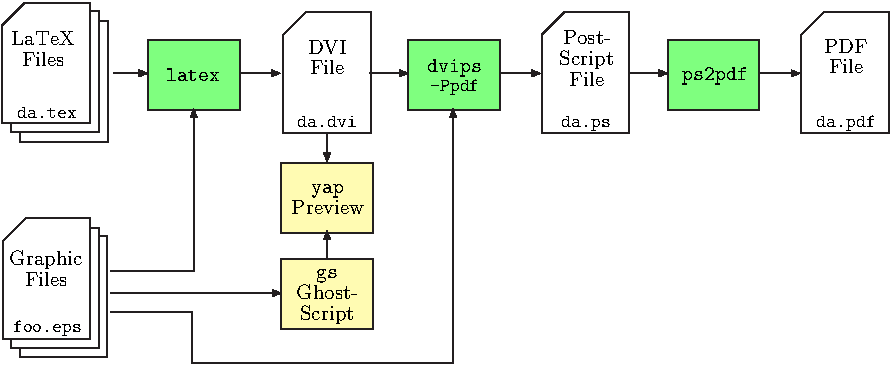
\includegraphics[width=1.0\textwidth]{workflow-cm}
\caption{Erzeugung von
PDF-Doku\-men\-ten im DVI-PS-Workflow. EPS-Grafiken werden erst bei der
Erzeugung der PS-Datei eingebunden. 
Anmerkung: Die abgebildete Vektorgrafik wurde mit \emph{Freehand} unter
Verwendung der \emph{BaKoMa} TrueType-Schriften erstellt %
(s.\ Abschn.\ \ref{sec:tex-schriften-in-grafiken}).}
\label{fig:latex-pdf-workflow}
\end{figure}

\end{comment}


\section{Drucken}

Vor dem Drucken der Arbeit empfiehlt es sich, einige Dinge zu beachten, um unnötigen Aufwand (und auch Kosten) zu vermeiden.

\subsection{Drucker und Papier}

Die Abschlussarbeit sollte in der Endfassung unbedingt auf einem
qualitativ hochwertigen Laserdrucker ausgedruckt werden, Ausdrucke
mit Tintenstrahldruckern sind \emph{nicht} ausreichend. Auch das
verwendete Papier sollte von guter Qualität (holzfrei) und
üblicher Stärke (mind.\ $80\; {\mathrm g} / {\mathrm m}^2$) sein.
Falls \emph{farbige} Seiten notwendig sind, sollte man diese einzeln%
\footnote{Tip: Mit \emph{Adobe Acrobat} lassen sich sehr einfach einzelne Seiten
des Dokuments für den Farbdruck auswählen und zusammenstellen.}
auf einem Farb-Laserdrucker ausdrucken und dem Dokument beifügen.

Übrigens sollten \emph{alle} abzugebenden Exemplare \textbf{gedruckt} (und nicht kopiert) werden! Die Kosten für den Druck
sind heute nicht höher als die für Kopien, der
Qualitätsunterschied ist jedoch -- \va\ bei Bildern und Grafiken
-- meist deutlich.


\subsection{Druckgröße}

Zunächst sollte sichergestellt werden, dass die in der fertigen PDF-Datei eingestellte
Papiergröße tatsächlich \textbf{A4} ist! Das geht \zB\ mit \emph{Adobe Acrobat}
oder \emph{SumatraPDF}
über \texttt{File} $\rightarrow$ \texttt{Properties},
wo die Papiergröße des Dokuments angezeigt wird:
\begin{center}
\textbf{Richtig:} A4 = $8{,}27 \times 11{,}69$ in \bzw\ $21{,}0 \times 29{,}7$ cm.
\end{center}
Falls das nicht stimmt, ist vermutlich irgendwo im Workflow versehentlich \textbf{Letter} 
als Papierformat eingestellt, %, häufig ist \emph{Adobe Distiller} "`schuld"'.


Ein häufiger und leicht zu übersehender Fehler beim Ausdrucken von
PDF-Doku\-menten wird durch die versehentliche Einstellung der
Option "`Fit to page"' im Druckmenü verursacht, wobei die Seiten
meist zu klein ausgedruckt werden. Überprüfen Sie daher die Größe
des Ausdrucks anhand der eingestellten Zeilenlänge oder mithilfe
einer Messgrafik, wie am Ende dieses Dokuments gezeigt.
Sicherheitshalber sollte diese Messgrafik bis zur
Fertigstellung der Arbeit beibehalten und die entsprechende
Seite erst ganz am Schluss zu entfernt werden.
Wenn, wie häufig der Fall, einzelne Seiten getrennt in Farbe gedruckt 
werden, so sollten natürlich auch diese genau auf die Einhaltung der Druckgröße 
kontrolliert werden!




\section{Binden}

Die Endfassung der Abschlussarbeit%
\footnote{Für \textbf{Bachelorarbeiten} genügt, je nach Vorgaben des Studiengangs, meist eine einfache Bindung (Copyshop oder Bibliothek).}
ist in fest gebundener Form
einzureichen.%
\footnote{An der Fakultät Hagenberg ist bei Masterarbeiten zumindest eines der
Exemplare \emph{ungebunden} abzugeben -- dieses wird später von einem
Buchbinder in einheitlicher Form gebunden und verbleibt
danach in der Bibliothek. Datenträger sind bei diesem Exemplar lose 
und \emph{ohne} Aufkleber (jedoch beschriftet) beizulegen.}
Dabei ist eine Bindung zu
verwenden, die das Ausfallen von einzelnen Seiten nachhaltig
verhindert, \zB durch eine traditionelle Rückenbindung
(Buchbinder) oder durch handelsübliche Klammerungen aus Kunststoff
oder Metall. Eine einfache Leimbindung ohne Verstärkung ist
jedenfalls \emph{nicht} ausreichend.


Falls man -- was sehr zu empfehlen ist -- die Arbeit bei einem
professionellen Buchbinder durchführen lässt, sollte man auch auf
die Prägung am Buchrücken achten, die kaum zusätzliche Kosten
verursacht. Üblich ist dabei die Angabe des Familiennamens des
Autors und des Titels der Arbeit. Ist der Titel der Arbeit zu
lang, muss man notfalls eine gekürzte  Version angeben, wie \zB:
%
\begin{center}
\setlength{\fboxsep}{3mm}
\fbox{
\textsc{Schlaumeier}
\textperiodcentered\ \textsc{Part.\ Lösungen zur allg.\ Problematik}}
\end{center}
%



\section{Elektronische Datenträger (CD-R, DVD, USB-Stick)}
Speziell bei Arbeiten im Bereich der Informationstechnik (aber
nicht nur dort) fallen fast immer Informationen an, wie Programme,
Daten, Grafiken, Kopien von Internetseiten \usw, die für eine
spätere Verwendung elektronisch verfügbar sein sollten.
Vernünftigerweise wird man diese Daten während der Arbeit bereits
gezielt sammeln und der fertigen Arbeit auf einer CD-ROM, DVD oder
einem USB-Stick beilegen. Es ist außerdem sinnvoll -- schon allein
aus Gründen der elektronischen Archivierbarkeit -- die eigene Arbeit
selbst als PDF-Datei beizulegen.%
\footnote{Auch Bilder und Grafiken könnten in elektronischer Form nützlich
sein, die \latex- oder Word-Dateien sind hingegen überflüssig.}


Falls ein elektronischer Datenträger (CD-ROM, DVD, USB-Stick) beigelegt
wird, sollte auf folgende Dinge geachtet werden:
%
\begin{enumerate}
\item Jedem abzugebenden Exemplar muss eine identische Kopie des
Datenträgers beiliegen. %
\item Verwenden Sie qualitativ hochwertige Rohlinge und überprüfen
Sie nach der Fertigstellung die tatsächlich gespeicherten Inhalte
des Datenträgers! %
\item Der Datenträger sollte in eine im hinteren Umschlag
eingeklebte Hülle eingefügt sein und sollte so zu entnehmen sein,
dass die Hülle dabei \emph{nicht} zerstört wird (die
meisten Buchbinder haben geeignete Hüllen parat). %
\item Der Datenträger muss so beschriftet sein, dass er der
Abschlussarbeit eindeutig zuzuordnen ist, am Besten durch ein
gedrucktes Label%
\footnote{Nicht beim lose abgegebenen Bibliotheksexemplar --
dieses erhält ein standardisiertes Label durch die Bibliothek.} %
oder sonst durch \emph{saubere}
Beschriftung mit
der Hand und einem feinen, wasserfesten Stift. %
\item Nützlich ist auch ein (grobes) Verzeichnis der Inhalte des
Datenträgers (wie exemplarisch in Anhang \ref{app:cdrom}).
\end{enumerate}

\chapter{Schlussbemerkungen}
\label{cha:Schluss}



%%%----------------------------------------------------------
\appendix                                            % Anhang 
%%%----------------------------------------------------------

\chapter{Technische Informationen}
\label{app:TechnischeInfos}

\newcommand*{\checkbox}{{\fboxsep 1pt%
\framebox[1.30\height]{\vphantom{M}\checkmark}}}

\section{Aktuelle Dateiversionen}

\begin{center}
\begin{tabular}{|l|l|}
\hline
Datum & Datei \\
\hline\hline
\hgbDate       & \texttt{hgb.sty} \\
\hline
\end{tabular}
\end{center}




\section{Details zur aktuellen Version}


Das ist eine völlig überarbeitete Version der DA/BA-Vorlage, die
\mbox{UTF-8} kodierten Dateien vorsieht und ausschließlich im PDF-Modus arbeitet.
Der "`klassische"' DVI-PS-PDF-Modus wird somit nicht mehr unterstützt! 

\subsection{Allgemeine technische Voraussetzungen}

Eine aktuelle \latex-Installation mit
\begin{itemize}
	
		\item Texteditor für \mbox{UTF-8} kodierte (Unicode) Dateien,
		\item \texttt{biber}-Programm (BibTeX-Ersatz, Version $\geq 1.5$),
		\item \texttt{biblatex}-Paket (Version $\geq 2.5$, 2013/01/10),
		\item Latin Modern Schriften (Paket \texttt{lmodern}).%
			\footnote{\url{http://www.ctan.org/pkg/lm}, \url{http://www.tug.dk/FontCatalogue/lmodern}}
\end{itemize}


\subsection{Verwendung unter Windows}
\label{sec:VerwendungUnterWindows}

Eine typische Installation unter Windows sieht folgendermaßen aus
(s.\ auch Abschnitt \ref{sec:Windows}):
%
\begin{enumerate}
\item \textbf{MikTeX 2.9}%
	\footnote{\url{http://www.miktex.org/} -- \textbf{Achtung:} 
	Generell wird die \textbf{Komplett\-installation} von MikTeX ("`Complete MiKTeX"') empfohlen, 
	da diese bereits alle notwendigen Zusatzpakete und Schriftdateien enthält! 
	Bei der Installation ist darauf zu achten, 
	dass die automatische Installation erforderlicher Packages 
	durch "`\emph{Install missing packages on-the-fly: = Yes}"' ermöglicht wird (NICHT "`\emph{Ask me first}"')!
	Außerdem ist zu empfehlen, unmittelbar nach der Installation von MikTeX mit dem Programm
	\texttt{MikTeX} $\to$ \texttt{Maintenance} $\to$ \texttt{Update} und \texttt{Package Manager} 
	ein Update der installierten Pakete durchzuführen.}
	(LaTeX-Basisumgebung),
\item \textbf{TeXnicCenter 2.0}%
	\footnote{\url{http://www.texniccenter.org/}}
	(Editor, unterstützt UTF-8),
\item \textbf{SumatraPDF}%
	\footnote{\url{http://blog.kowalczyk.info/software/sumatrapdf/}} 
	(PDF-Viewer).
\end{enumerate}
%
Ein passendes TeXnicCenter-Outputprofil für MikTeX, Biber und Sumatra ist in diesem Paket enthalten.%
\footnote{Datei \nolinkurl{_setup/texniccenter/tc_output_profile_sumatra_utf8.tco}} 
Dieses sollte man zuerst
über \texttt{Build} $\to$ \texttt{Define Output Profiles...} in TeXnicCenter importieren.
\textbf{Achtung}: Alle neu angelegten \texttt{.tex}-Dateien sollten grundsätzlich in UTF-8 Kodierung gespeichert werden!


\subsection{Verwendung unter Mac~OS}

Diese Version sollte insbesondere mit \emph{MacTeX} problemlos laufen (s.\ auch Abschnitt \ref{sec:MacOs}):
\begin{enumerate}
\item 
	\emph{MacTex} (2012 oder höher).
\item 
	Die Zeichenkodierung des Editors sollte auf UTF-8 eingestellt sein.
\item 
	Als Engine (vergleichbar mit den Ausgabeprofilen in TeXnicCenter) sollte \emph{LaTeXMk} verwendet werden. 
	Dieses Perl-Skript erkennt automatisch, wie viele Aufrufe von \emph{pdfLaTeX} und \emph{Biber} nötig sind. 
	Die Ausgabeprofile \emph{LaTeX} oder \emph{pdfLaTeX} hingegen müssen mehrmals aufgerufen werden, 
	zudem werden hierbei auch die Literaturdaten nicht verarbeitet. Dazu müsste extra die \emph{Biber}-Engine 
	aufgerufen werden, 	die jedoch noch nicht in allen Editoren vorhanden ist.
\end{enumerate}
	% Technische Ergänzungen
\chapter{Inhalt der CD-ROM/DVD}
\label{app:cdrom}

\paragraph{Format:} 
		CD-ROM, Single Layer, ISO9660-Format%
\footnote{Verwenden Sie möglichst ein Standardformat, bei DVDs natürlich
eine entsprechende andere Spezifikation.}


\section{PDF-Dateien}
\begin{FileList}{/}
%\fitem{_DaBa.dvi} Gesamtdokument (DVI-File, ohne Grafiken)
\fitem{_thesis_DE.pdf} Master- oder Bachelorarbeit mit Instruktionen (Gesamtdokument)
\fitem{_praktikum.pdf} Praktikumsbericht (verkürzte Version der Bachelorarbeit) %
\end{FileList}


\section{\latex-Dateien}

\textbf{Achtung:} Die folgende Auflistung soll nur den Gebrauch dieser Vorlage erleichtern. Es ist bei einer Master- oder Bachelorarbeit \ia\ \emph{nicht} notwendig, die zugehörigen \latex-Dateien aufzulisten (wohl aber projektbezogene Dateien, Ergebnisse, Bilder, Kopien von Online-Literatur etc.)!

\begin{FileList}{/}
\fitem{_thesis_DE.tex} Master-/Bachelorarbeit (Hauptdokument) %
\fitem{_praktikum.tex} Praktikumsbericht (verkürzte Version der Bachelorarbeit) %
\fitem{references.bib} Literatur-Datenbank (BibTeX-File)
\end{FileList}

\begin{FileList}{/thesis_DE/front}
\fitem{vorwort.tex} Vorwort %
\fitem{kurzfassung.tex} Kurzfassung %
\fitem{abstract.tex} Abstract %
\end{FileList}

\begin{FileList}{/thesis_DE/chapters}
\fitem{einleitung.tex} Kapitel 1 %
\fitem{diplomschrift.tex} Kapitel 2 %
\fitem{latex.tex} Kapitel 3
\fitem{abbildungen.tex} Kapitel 4 %
\fitem{formeln.tex} Kapitel 5 %
\fitem{literatur.tex} Kapitel 6 %
\fitem{drucken.tex} Kapitel 7 %
\fitem{word.tex} Kapitel 8 %
\fitem{schluss.tex} Kapitel 9 %
\end{FileList}

\begin{FileList}{/thesis_DE/back}
\fitem{anhang_a.tex} Anhang A (Source Code) %
\fitem{anhang_b.tex} Anhang B (Inhalt CD-ROM) %
\fitem{anhang_c.tex} Anhang C (Liste der Änderungen) %
\fitem{anhang_d.tex} Anhang D (LaTeX-Quellcode) %
\fitem{messbox.tex} Messbox zur Druckkontrolle %
\end{FileList}

\section{Style/Class-Dateien}

\begin{FileList}{/}
\fitem{hgbthesis.cls} LaTeX Class-Datei für Master- und Bachelorarbeiten
\fitem{hgb.sty} LaTeX Style-Datei für alle Hagenberg-Dokumente
\fitem{hgbabbrev.sty} LaTeX Style-Datei mit Abkürzungs-Makros
\fitem{hgbbib.sty} LaTeX Style-Datei mit Bibiographie-Einstellungen
\fitem{hgbheadings.sty} LaTeX Style-Datei für Überschriften
\fitem{hgblistings.sty} LaTeX Style-Datei für Code-Umgebungen
\end{FileList}


\section{Sonstiges}

\begin{FileList}{/images}
\fitem{*.ai} Original Adobe Illustrator-Dateien %
\fitem{*.fh11} Original Macromedia Freehand-Dateien %
\fitem{*.jpg, *.png} Original Rasterbilder %
\end{FileList}
	% Inhalt der CD-ROM/DVD
\chapter{Fragebogen}
\label{app:Fragebogen}

	% Chronologische Liste der Änderungen
\chapter{\latex-Quellkode}
\label{app:latex}

\section*{Hauptdatei \texttt{\_thesis\_DE.tex}}

\paragraph{Anmerkung:}
Das sollte nur ein \emph{Beispiel} für die Einbindung von Quellcode
in einem Anhang sein. Der \latex-Quellkode der eigenen
Abschlussarbeit ist meist \emph{nicht} interessant genug, um ihn hier
wiederzugeben!

\begin{footnotesize}
\verbatiminput{_thesis_DE.tex}
\end{footnotesize}





	% Quelltext dieses Dokuments

%%%----------------------------------------------------------
\MakeBibliography                        % Quellenverzeichnis
%%%----------------------------------------------------------

%%% Messbox zur Druckkontrolle ------------------------------
\chapter*{Messbox zur Druckkontrolle}



\begin{center}
{\Large --- Druckgröße kontrollieren! ---}

\bigskip

\calibrationbox{100}{50} % Angabe der Breite/Hoehe in mm

\bigskip

{\Large --- Diese Seite nach dem Druck entfernen! ---}

\end{center}



%%%----------------------------------------------------------
\end{document}
%%%----------------------------------------------------------